
%% 歩容パターンの再評価手法の提案.tex
%% LaTeX-2e 専用

%% 全体の流れとしては,まず,先行研究の問題点を指摘し,次に,歩容パターンの再評価手法を提案する.

\chapter{歩容パターンの再評価手法の提案}\label{chapter:歩容パターンの再評価手法の提案}
第\ref{chapter:歩容パターンの再評価手法の提案}章では,先行研究の手法およびその問題点を指摘し,
常に脚軌道生成が可能な自由歩容パターン生成手法として,歩容パターンの再評価手法を述べる.

% 先行研究の章
\section{本研究室における自由歩容パターン生成の先行研究}
最初にグラフ探索よる自由歩容パターン生成手法において用いる用語を定義し,
先行研究で行われてきた自由歩容パターン生成手法について述べる.
また,先行研究で用いられてきた自由歩容パターン生成手法の問題点について述べる.

\subsection{グラフ理論について}
本論文ではグラフ理論を用いた自由歩容パターン生成手法を論ずるため,まずはグラフ理論について説明をする.
グラフとは,頂点(ノード)とそれらを結ぶ辺(エッジ)からなる図形である.
このグラフを用いて,さまざまな問題を取り扱う学問をグラフ理論という.

以降の説明を簡単にするため,この論文で用いるグラフ理論の用語について簡潔に述べる.
グラフ上のあるノードから別のノードにエッジを用いて移動することを遷移と呼ぶ.
遷移の際,移動前のノードを始点,移動後のノードを終点と呼ぶ.
グラフの種類は大別して有向グラフと無向グラフに分けられ,
エッジに向きがあるものを有向グラフ(\figref{fig:directed_graph}),
逆に向きを持たないものを無向グラフ(\figref{fig:undirected_graph})という.
また,閉路を持たず,かつ,すべてのノード間にエッジが存在するグラフを木という.
このような木構造をもつグラフのうち,\figref{fig:tree_graph}のように,
根となるノードを持ち,そのノードからすべてのノードに到達可能なものを根付き木という.
根付き木を図形として表現する場合は簡単のため,
\figref{fig:tree_graph}のように根を上部に配置することが多い.

根付き木には無向グラフと有向グラフの2種類が存在するが,
後述する歩行パターングラフは有効グラフであるため,
有向の根付き木について説明を行う.
根付き木のエッジが,根が始点となるように伸びている場合,
あるノードから遷移可能なノードをそのノードの子ノードと呼ぶ.
逆に,あるノードに遷移可能なノードをそのノードの親ノードと呼ぶ.
親ノードを持たないノードを根ノードと呼び,子ノードを持たないノードを葉ノードと呼ぶ.
また,あるノードから根ノードまでのエッジの数をそのノードの深さと呼び,
根ノード自身の深さは0となる.

たとえば\figref{fig:tree_graph}において,ノードAが根ノードであり,ノードB,Cがその子ノードである.
また,ノードB,ノードD,E,ノードCはノードFを子ノードとして持ち,ノードD,E,Fは葉ノードである.
ノードAの深さは0であり,ノードB,Cの深さは1,ノードD,E,Fの深さは2となる.

\begin{figure}[h]
  \subfigure[Undirected Graph]{%
  \label{fig:undirected_graph}
  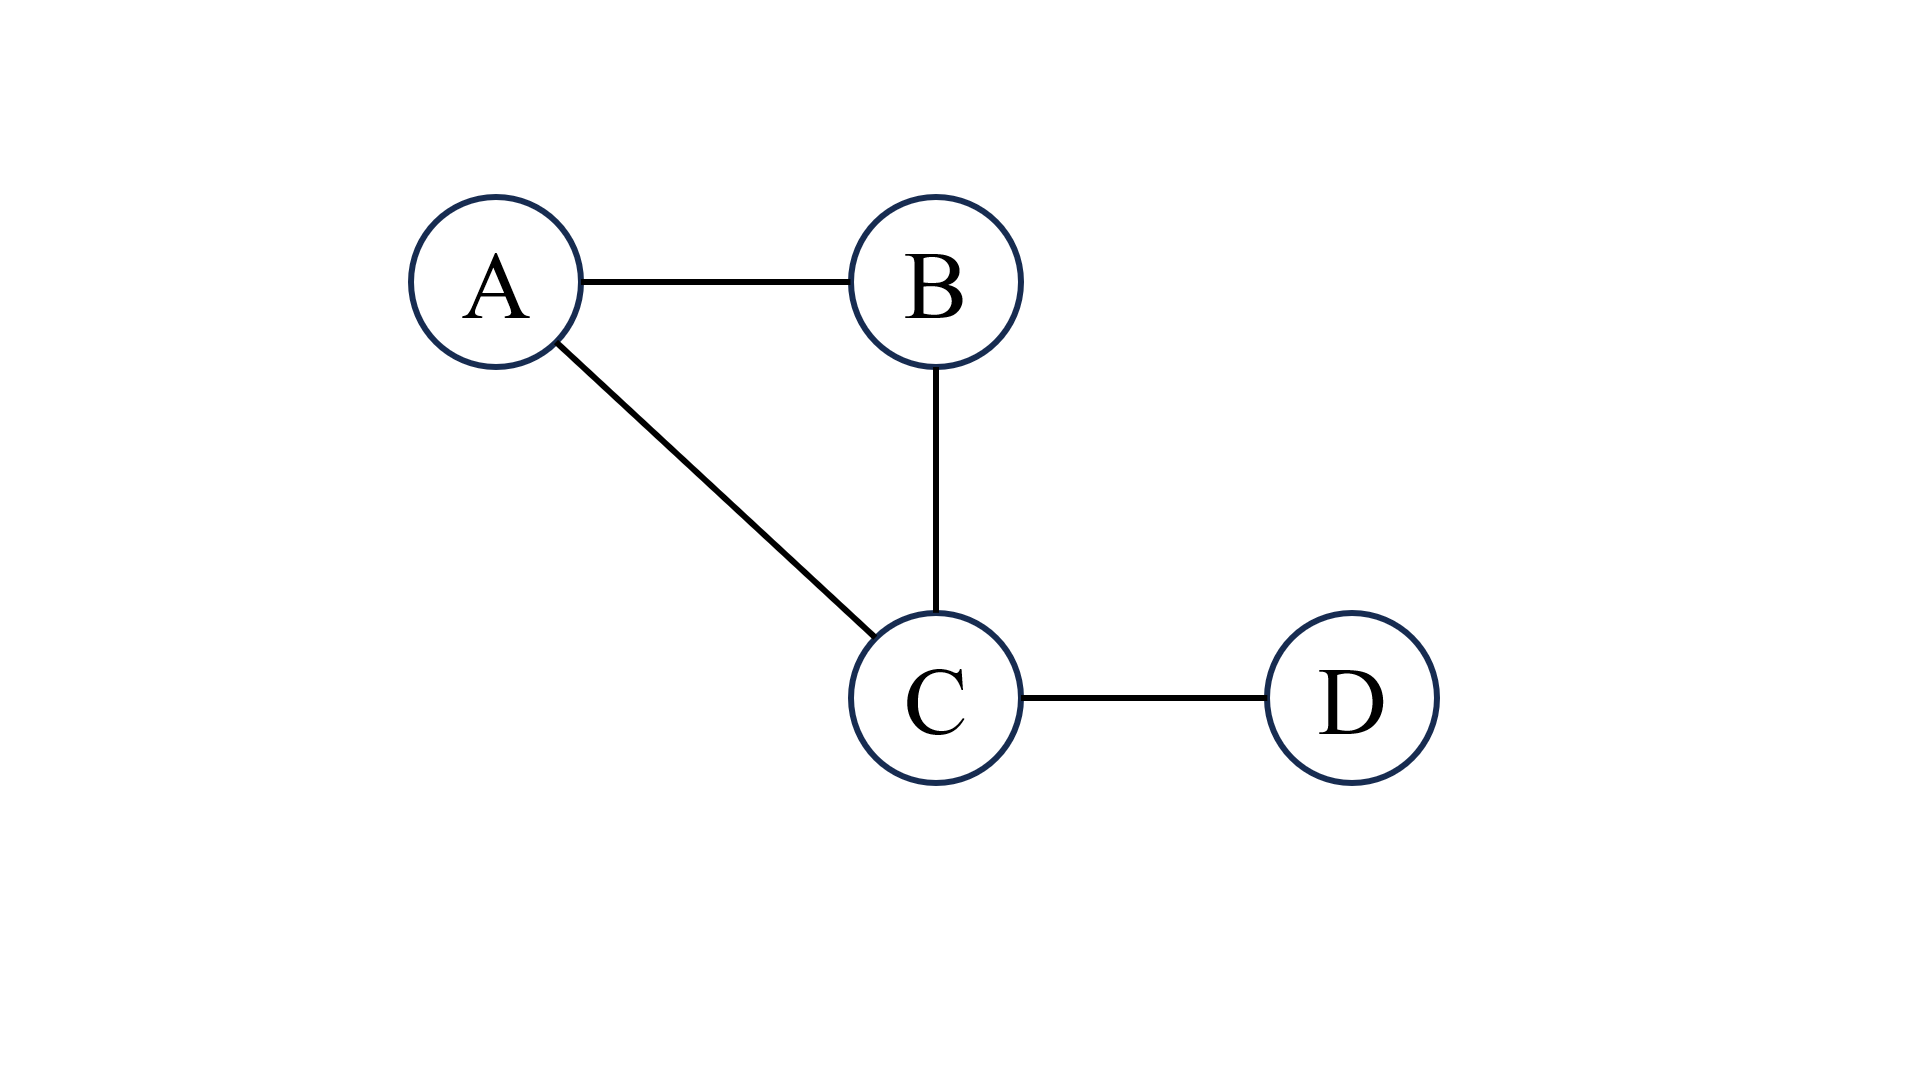
\includegraphics[width=0.48\columnwidth]{figure/chapter2/undirected_graph.png}}
  \hspace{0.02\columnwidth}
  \subfigure[Directed Graph]{%
  \label{fig:directed_graph}
  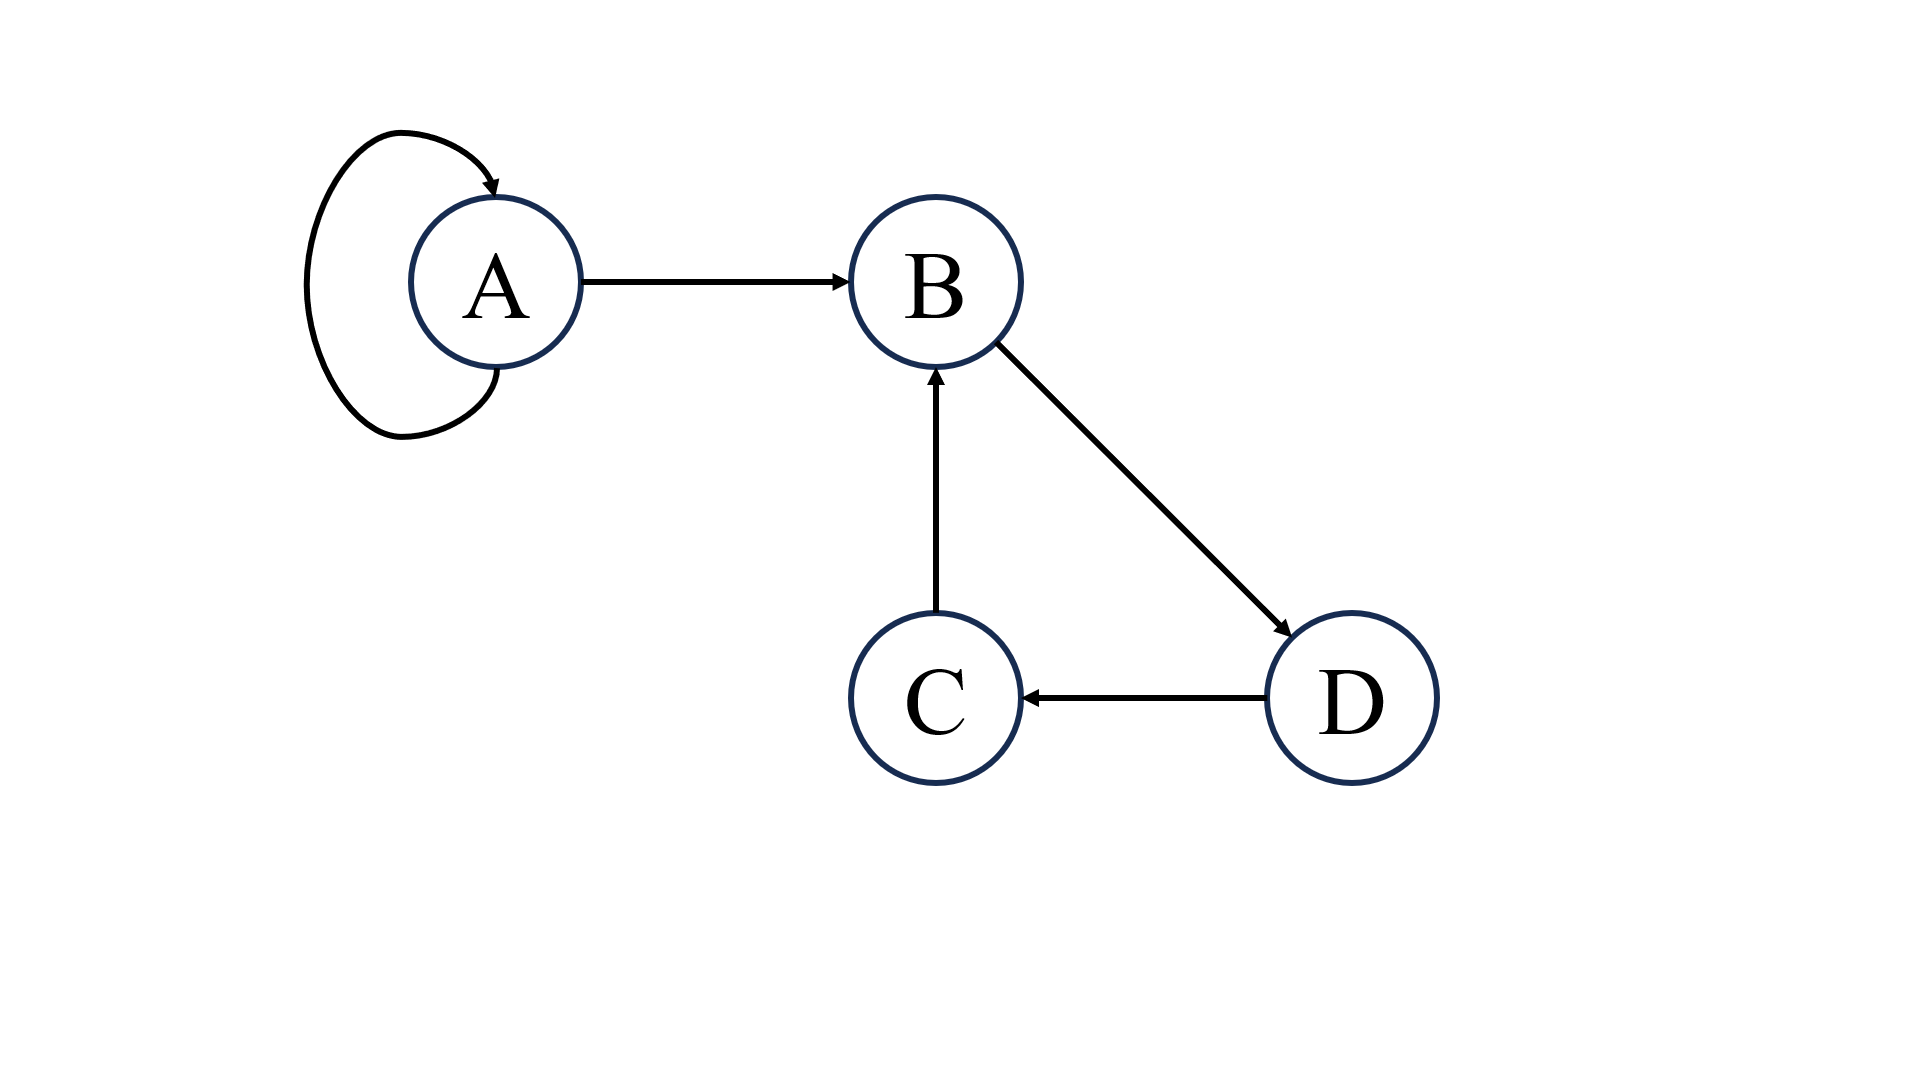
\includegraphics[width=0.48\columnwidth]{figure/chapter2/directed_graph.png}}
  \caption{Examples of simple graphs}
  \label{fig:example_simple_graphs}  % chktex 24
\end{figure}

\begin{figure}[h]
  \begin{center}
    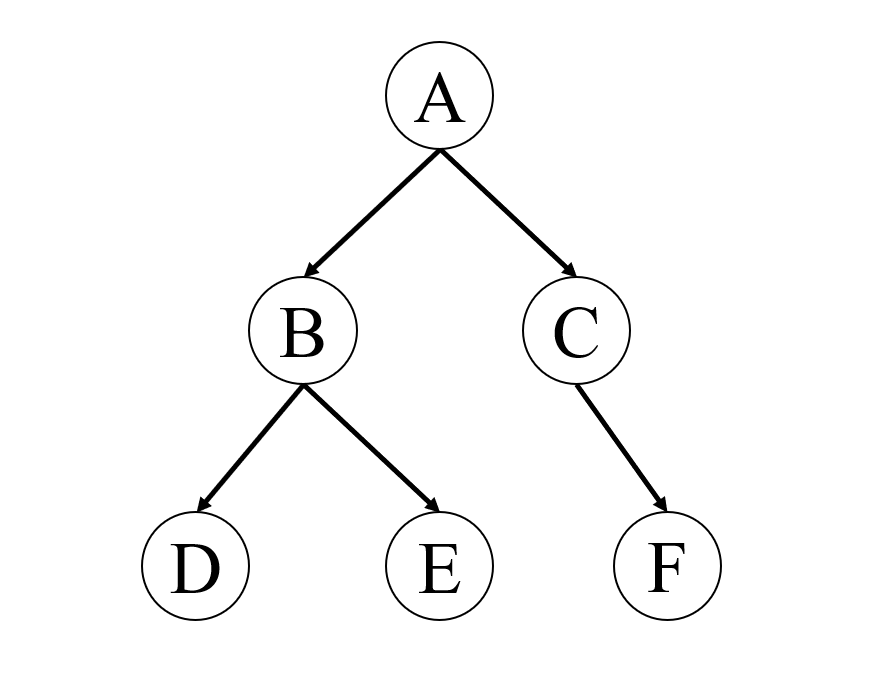
\includegraphics[width=50mm, clip]{figure/chapter2/tree_graph.png}
    \caption{Tree Graph}
    \label{fig:tree_graph} % chktex 24
  \end{center}
\end{figure}

グラフのあるノードから別のノードに到達するための経路をパスと呼び,
これを求めることをグラフ探索と呼ぶ.
グラフ探索には,深さ優先探索,幅優先探索などのさまざまなアルゴリズムが存在する.
深さ優先探索では,始点となるノードから,深さが深くなる方向を優先して探索を行う.
これに対して,幅優先探索では,始点となるノードから,深さが浅いノードを優先して探索を行う手法である.

\subsection{歩容パターングラフの定義}
本研究においては,6脚ロボットの歩容パターンをグラフを用いて表現する.
グラフはロボットの状態をノードとし,ロボットの状態間の遷移,つまりロボットの動作をエッジとして作成する.
グラフは有向の根付き木とし,現在のロボットの状態を根ノード,
その姿勢から1動作で到達できる姿勢を子ノードとして根ノードに接続する.
また,このようにして作られたグラフを歩容パターングラフと定義する.
\figref{fig:image_of_gait_pattern_graph}に歩容パターングラフのイメージを示した.

本手法では,まず歩容パターングラフを作成する.
そして,根ノードから最適な動作を行う葉ノードまでのパスをグラフ探索によって求め,
そのパスに含まれる深さ1のノードを次の動作としてロボットに実行させる.
これを繰り返すことで,ロボットの歩容パターンを生成しているのである.

グラフ探索による歩容パターン生成においては,網羅的にロボットの状態を調べ上げるため,
実時間内の計算を行うにはグラフの規模を小さくすることが求められる.
しかし,歩容パターングラフはロボットの状態や動作を対象とするため無数の組み合わせが存在し,
そのすべてを網羅的に調べ上げることは困難である.
そのため,状態や動作を離散化することで歩容パターン生成をグラフへ落とし込む必要がある.
以下に各要素の離散化方法について述べる.
\\  % 1行開ける

\begin{figure}[h]
  \begin{center}
    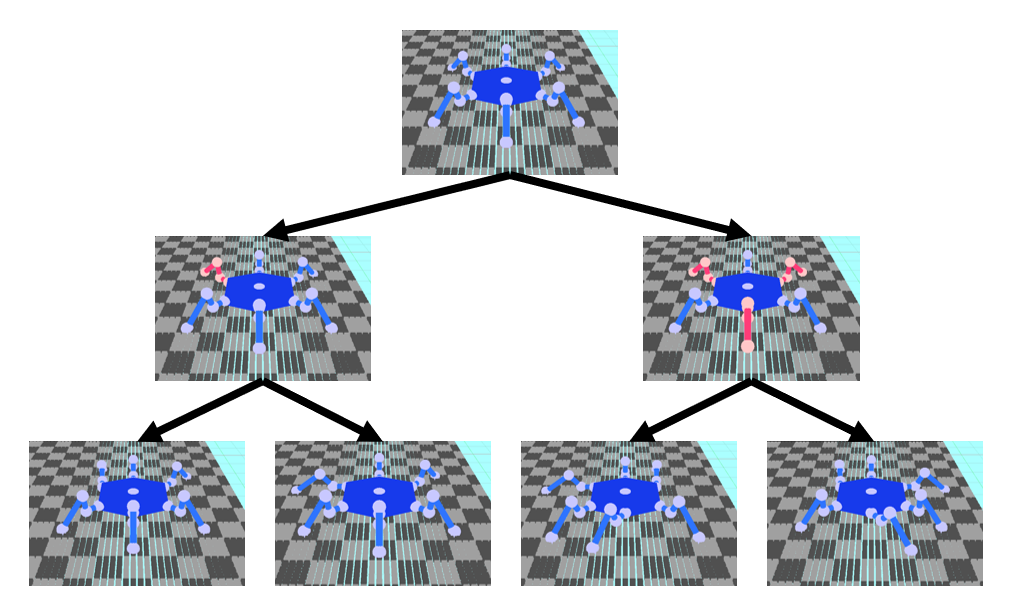
\includegraphics[width=100mm, clip]{figure/chapter2/gait_pattern_graph.png}
    \caption{Image of Gait Pattern Graph}
    \label{fig:image_of_gait_pattern_graph} % chktex 24
  \end{center}
\end{figure}

\subsubsection{グラフの階層構造}
前述のとおり,ロボットの脚位置は脚の可動範囲内であれば,無数の位置を取ることができる.
そのため本手法では,基準となる脚位置を決め,その基準からの相対位置を用いて脚位置を離散化している.
Prabirらが提案した手法では2次元平面での移動を前提としていたが\cite{Prabir_Graph_search},
これを三浦が3次元空間へ拡張した\cite{Miura_Graph_search}.

\figref{fig:discretization}に支持脚の脚位置の離散化の様子を示した.
\figref{fig:discretization}のように脚位置の基準座標を4とし,
脚位置4と同じ高さにあるかつ,進行方向に対して基準位置よりも前方にある脚位置を6,後方にある脚位置を2とする.
また,脚位置6よりも高い位置にある脚位置を7,低い位置にある脚位置を5とし,
脚位置2よりも高い位置にある脚位置を3,低い位置にある脚位置を1とする.
このようにして,脚位置を7つに離散化している.
遊脚している脚の脚位置は,支持脚の脚位置1$\sim$7に対応させ,脚位置1'$\sim$7'とする.% $\sim$ で波線を引く

これにより,脚位置1$\sim$7から脚位置1'$\sim$7'への遷移によって,脚の上下運動を表現することができる.
また,脚位置1'$\sim$7'内での遷移によって,遊脚の水平方向の移動を表現することができる.
以上より,脚の上下運動と脚の水平方向の移動をグラフで表現することができることを示した.

\begin{figure}[h]
  \begin{center}
    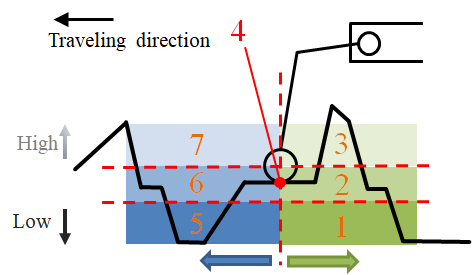
\includegraphics[width=75mm, clip]{figure/chapter2/discretization_of_leg_pos.png}
    \caption{Discretization of Leg Posistion}
    \label{fig:discretization} % chktex 24
  \end{center}
\end{figure}

このような脚位置の離散化を行うことで,脚位置の組み合わせを有限個に抑えることができるが,
脚位置の組み合わせは未だ,$7^6 = 117649 \approx 10^5$通り存在し,
遊脚である時を含めるとさらに組み合わせが増えてしまうことがわかる.
プログラムの実行環境によって左右されるが,
プログラミング言語のC++で作成した処理では約1秒間に$10^8$回程度の計算が可能であるとされており\cite{Program_Challenge_Book},
この組み合わせをすべて歩容パターングラフに追加した場合,実時間内の処理を行うにはグラフの規模が大きくなりすぎる.
そこで,大木らは脚位置の組み合わせを階層構造化することで,
遊脚時の脚位置1'$\sim$7'を省略し,探索するノード数を減らすことに成功した\cite{Oki_Graph_search}.

階層構造とこれを利用した探索の方法を説明するために,遊脚の組み合わせと脚位置の組み合わせについて定義を行う.
遊脚の組み合わせは,ロボットの各脚について,その脚が遊脚であるか支持脚であるかを表すノードの要素である.
6脚ロボットの右前脚を1番目の脚として,時計回りに2番目の脚から6番目の脚とする.
この時,i番目の脚が支持脚であることを$v_i = 1$,遊脚である時を$v_i = 0$とすると,
遊脚の組み合わせ$V$は\eqref{eq:leg_com}のように表すことができる.

\begin{equation}\label{eq:leg_com}
  V = \{v_1, v_2, v_3, v_4, v_5, v_6\}
\end{equation}

\noindent 遊脚の組み合わせは$2^6 = 64$通り存在するが,
6脚,5脚,4脚が遊脚である組み合わせや,
隣り合う3脚が遊脚である組み合わせは
実際には取りえない組み合わせであるため,
探索するべき組み合わせは$2^6 - {}_6 \mathrm{C}_6 - {}_6 \mathrm{C}_5 - {}_6 \mathrm{C}_4 - 6 = 36$通りとなる.

また,脚位置の組み合わせとは離散化した脚位置において,各脚がどの位置にあるかを表すノードの要素である.
i番目の脚が脚位置jにあることを$k_i = j$とすると,
脚位置の組み合わせ$K$は\eqref{eq:leg_pos}のように表すことができる.

\begin{equation}\label{eq:leg_pos}
  K = \{k_1, k_2, k_3, k_4, k_5, k_6\}
\end{equation}

\noindent\eqref{eq:leg_com},\eqref{eq:leg_pos}より
ロボットの脚の状態は遊脚の組み合わせ$V$と脚位置の組み合わせ$K$を用いて表すことができるようになった.
i番目の脚の状態を$l_i = v_i \cdot k_i$とすると,$L$は\eqref{eq:leg_state}のように表すことができる.

\begin{equation}\label{eq:leg_state}
  L_{ij} = \{v_1 \cdot k_1, v_2 \cdot k_2, v_3 \cdot k_3, v_4 \cdot k_4, v_5 \cdot k_5, v_6 \cdot k_6\}
\end{equation}

\noindent\eqref{eq:leg_state}より,脚位置の組み合わせが$K = \{1,1,1,1,1,1\}$で
遊脚の組み合わせが$V = \{0,1,0,1,0,1\}$である時の脚の状態を$L_{ij} = \{0,1,0,1,0,1\}$と表すことができる.
同様に,脚位置の組み合わせが$K = \{3,1,3,1,3,1\}$で遊脚の組み合わせが$V = \{0,1,0,1,0,1\}$である時の脚状態は
$L_{ij} = \{0,1,0,1,0,1\}$と表すことができる.
このことから,ある脚位置の組み合わせから,別の脚位置の組み合わせへの遷移は,
脚の状態$L$が等しいときのみ可能であることがわかる.

以上の定義より,階層構造と階層を用いたグラフの探索方法について説明することができる.
階層とは脚位置の組み合わせ$K$が等しく,かつ,遊脚の組み合わせ$V$が異なるノードの集合と定義され,
遊脚の組み合わせが36通り存在することから,同じ階層内のノードは36個存在する.
脚の上下運動を実現したい場合は,遊脚の組み合わせ$V$が異なるノードを探索する必要があるため,
図\ref{fig:hierarchy2}のように階層内のノード36個のみを探索すればよい.

また,脚の水平運動を実現したい場合は,脚位置の組み合わせ$K$が異なるノードを探索する必要があるため,
図\ref{fig:hierarchy}のように脚の状態$L$が等しくなるノードのみを探索すればよい.
脚の状態$L$が等しくなるノードは,最大で3脚が遊脚しているときの$7^3 = 343$個であるため,
十分に実時間内の計算が可能である.

\begin{figure}[htbp]
  \begin{center}
    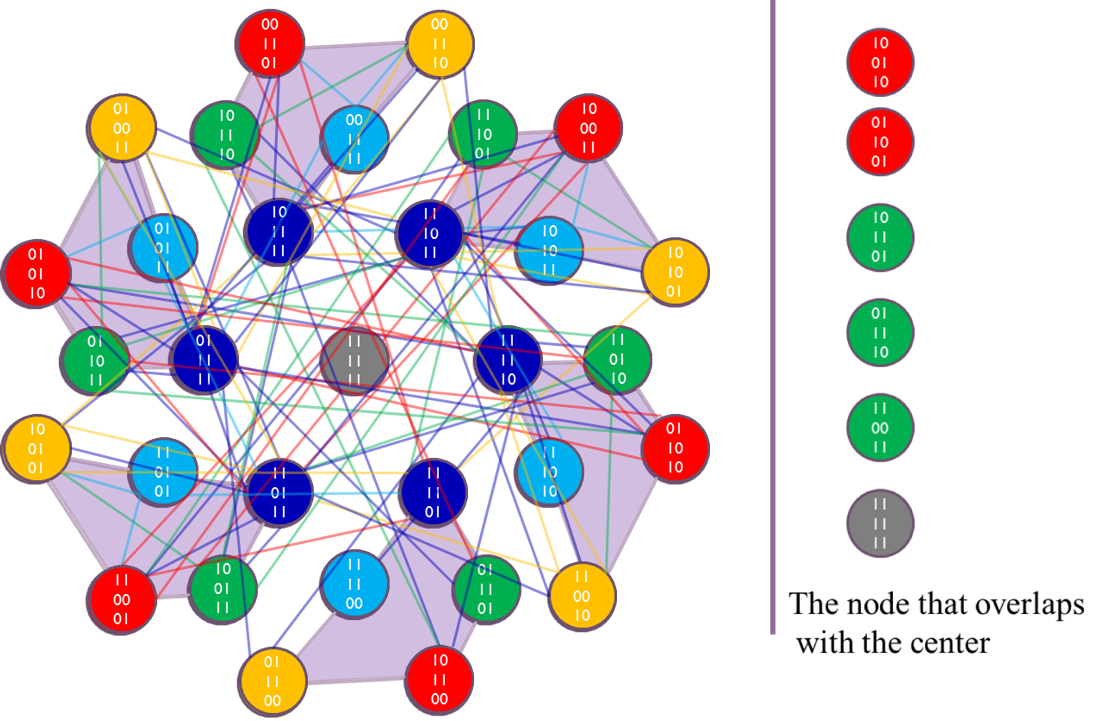
\includegraphics[width=75mm, clip]{figure/chapter2/hierarchy2.png}
    \caption{Search in the Same Hierarchy}
    \label{fig:hierarchy2} % chktex 24
  \end{center}
\end{figure}

\begin{figure}[htbp]
  \begin{center}
    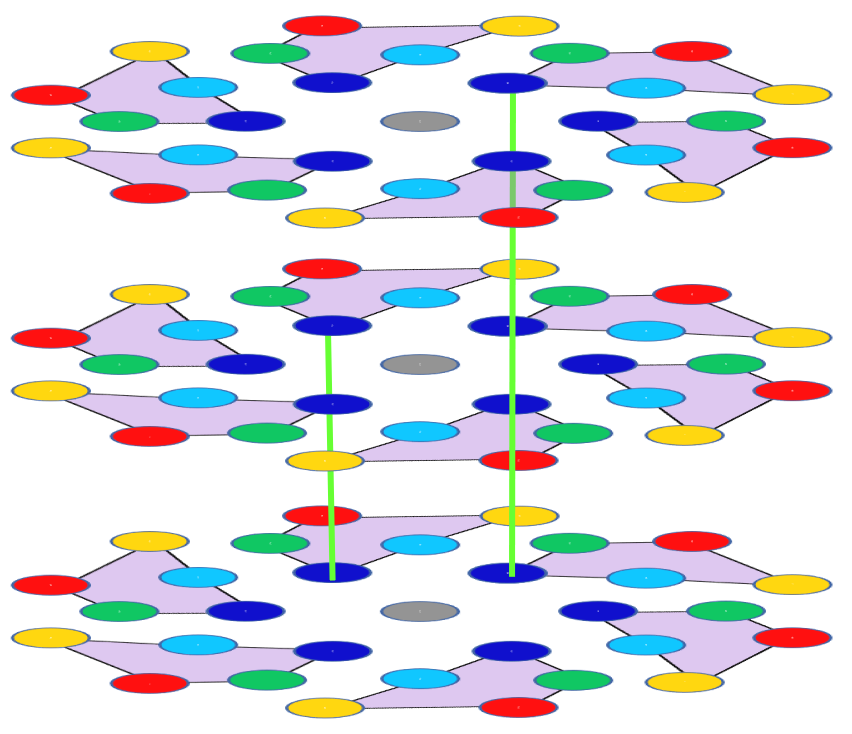
\includegraphics[width=75mm, clip]{figure/chapter2/hierarchy.png}
    \caption{Search in the Difficult Hierarchy}
    \label{fig:hierarchy} % chktex 24
  \end{center}
\end{figure}

\subsubsection{脚軌道生成の分離}
次に歩容パターングラフのエッジについて述べる.
歩容パターングラフにおいて,エッジはロボットの動作を表す.
ロボットの動作は脚の接地・遊脚運動と,重心の移動からなるため,これらの動作に対応するエッジを作成する.
具体的には,脚の上下移動のエッジ,脚の水平移動のエッジ,重心の上下移動のエッジ,
重心の水平移動のエッジ,そして,重心の回転のエッジを用いてロボットの動作を表現する.

これらのエッジには,移動前と移動後のノードを補完するための状態を持っておらず,
単純に移動前と移動後のノードを結ぶのみである.
これはつまり,歩容パターングラフを生成するプログラムと,脚軌道を生成するプログラムが分離されていることを意味する.
脚軌道を考える場合,ロボットの関節の可動範囲を考慮する必要があり,逆運動学解を用いる脚の関節角度の計算が求められる.
しかし,逆運動学の計算には計算負荷の大きい逆三角関数の計算が必要となり,各エッジについて網羅的に計算を行うことを考えると,
実時間内の計算が困難になってしまう.
そのため本手法では,歩容パターングラフを生成するプログラムを分離し,
歩容パターングラフの生成時には脚の可動範囲は近似的な値を用いて計算することで,
実時間内の計算を可能にしている.

近似された脚の可動範囲の求め方について述べる.
近似された脚の可動範囲は脚の付け根を中心とする環状の扇形として表現する.
簡単のため,以降は扇形の外径を最大半径,内径を最小半径と呼ぶことにする.
まず,脚先を届くことができる範囲を求めるために,
最大半径を以下の手順で求める.
\begin{enumerate}
  \item 脚の付け根と脚先が同じ高さになるように脚先を上げる.
  \item 図\ref{fig:leg_range_a}のように水平方向に脚先を$1 [mm]$ずつ伸ばす.
  \item 脚先を伸ばすことができなくなった場合,\\
        図\ref{fig:leg_range_b}のように脚先と脚の付け根の高さ方向の距離の差をインデックスとして,\\
        脚先と第1関節の水平方向の距離を最大半径として記録する.
  \item 脚先を$1 [mm]$下げて(2)(3)の処理を繰り返す.脚先を下げることができなくなった場合,処理を終了する.
\end{enumerate}
次に最小半径をロボットの脚長などのパラメータから決定する.
先行研究では実験で用いたロボットにあわせ,$120 [mm]$とした.
そして,扇形の中心角を隣の脚と干渉しないように決定する.
こうして求められる近似された脚の可動範囲のイメージを\figref{fig:approximated_range_of_motion}に示す.
\figref{fig:approximated_range_of_motion}では右中央の脚の近似された脚の可動範囲のみを示しており,
赤い領域で示される図形が近似された脚の可動範囲である.

このように近似を行ったことで,以下に示す手順で脚先が脚の可動範囲内にあるか判定することができる.
\begin{enumerate}
  \item 脚の付け根から脚先までの水平方向のベクトルを求め,ベクトルの傾きが扇形の中心角の範囲内にあるか判定する.
  \item 脚の付け根から脚先までの水平方向の距離を求める.
  \item 最小半径よりも大きく,最大半径よりも小さいか判定する.
  \item 以上の条件を満たす場合,脚先は脚の可動範囲内にあると判定する.
\end{enumerate}
(2)(3)の手順は四則演算のみで計算が可能であり,
(1)の手順もベクトルの内積を用いて計算が可能であるため同様に四則演算のみで計算が可能である.
そのため,脚先が脚の可動範囲内にあるかの判定を高速に行うことができる.
本手法では脚軌道生成だけでなく,脚の接地判定にもこの近似的な脚の可動範囲を用いている.


\begin{figure}[htbp]
  \subfigure[Horizontal Movement of the Leg Tips]{%
  \label{fig:leg_range_a}
  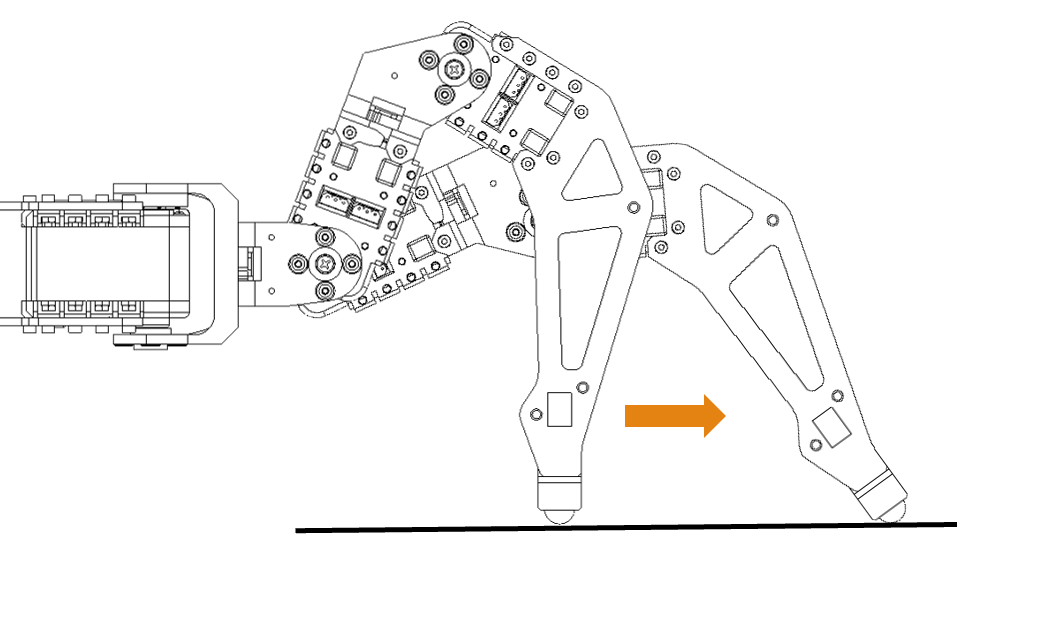
\includegraphics[width=0.48\columnwidth]{figure/chapter2/leg_range.png}}
  \hspace{0.04\columnwidth}
  \subfigure[Determination of the Maximum Radius]{%
  \label{fig:leg_range_b}
  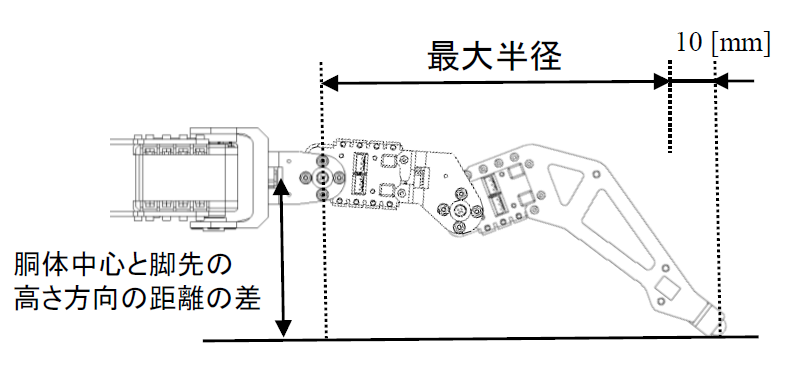
\includegraphics[width=0.48\columnwidth]{figure/chapter2/max_leg_range.png}}
  \caption{Caluculation of the Maximum Radius}
  \label{fig:leg_range}  % chktex 24
\end{figure}

\begin{figure}[htbp]
  \subfigure[Side View]{%
  \label{fig:side_view}
  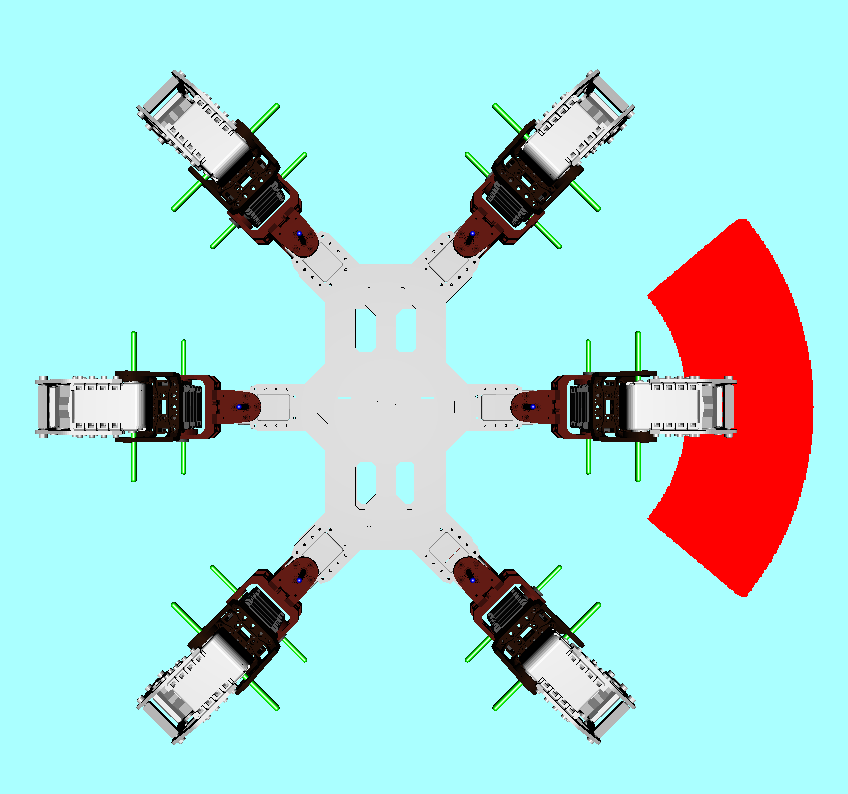
\includegraphics[width=0.48\columnwidth]{figure/chapter2/approximated_range_motion_top.png}}
  \hspace{0.04\columnwidth}
  \subfigure[Top View]{%
  \label{fig:top_view}
  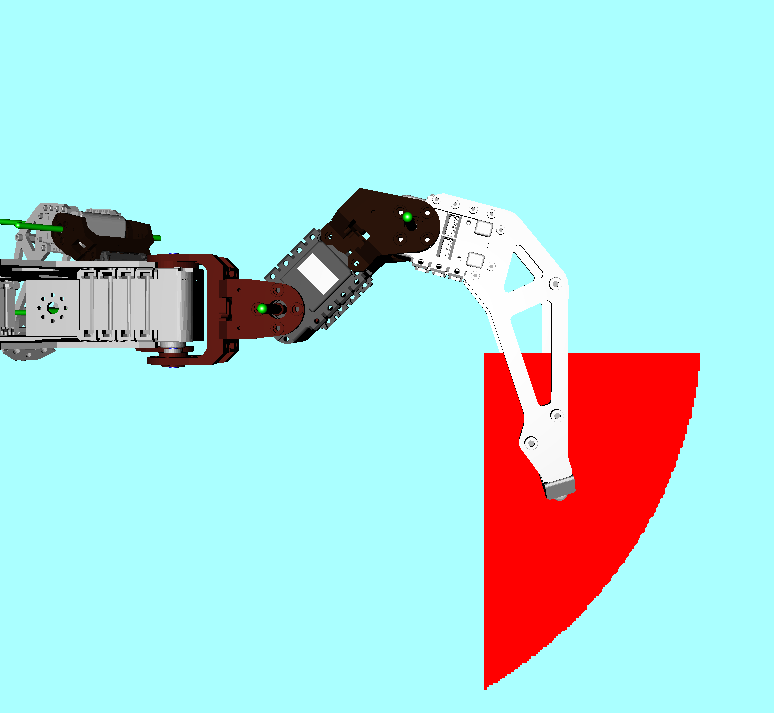
\includegraphics[width=0.48\columnwidth]{figure/chapter2/approximated_range_motion_back.png}}
  \caption{Approximated Range of Motion}
  \label{fig:approximated_range_of_motion}  % chktex 24
\end{figure}

\subsection{脚軌道生成の失敗}
先行研究ではグラフの階層構造化および脚軌道生成の分離によって,実時間内の計算が可能になった.
しかし,実際に実機を用いて歩行実験を行ったところ,低頻度ではあるが脚軌道生成に失敗することがあった.
失敗の原因として,脚の可動範囲に近似的な値を用いていることが予想される.
近似的な脚の可動範囲の境界近くは,実際には脚の可動範囲外であるが,
近似的な値を用いているために脚の可動範囲内と判定されてしまっている領域があると考えられる.
そのため,脚軌道や脚の接地点が脚の可動範囲外になってしまい,脚軌道生成に失敗することがあると考えられる.

失敗の原因についてより具体的に議論するために,脚の可動範囲の解析を行ったため,
その方法と結果を示す.
解析の対象とするロボットは,Trossen Robotics社のPhantomX Mark I\hspace{-1.2pt}I \cite{cita:phantom_x_mark_2}  % chktex 2
(以下PhantomX)とする.
PhantomX(\figref{fig:phantomx_mk2})は6脚ロボットであり,各脚に3つのアクチュエータを持つ.
また,関節配置は脚の付け根からヨー・ピッチ・ピッチの順である.

PhantomXの脚の可動範囲を求めるために,間接角度の逆運動解を求める式を導く.
まず,\figref{fig:leg_coordinate_axis}にPhantomXの脚の座標系を示す.
第1関節を原点とし,
x軸をロボットの前方方向にとり,z軸をロボットに垂直で上向きにとる.
y軸は右手座標系となるように設定する.
また簡単のため,解析には\figref{fig:joint_and_link}のようにPhantomXのアクチュエータの回転軸を結んだ仮想的なリンクを用いる.
リンク名は第1関節からCoxa Link,Femur Link,Tibia Linkであり,関節名はCoxa Joint,Femur Joint,Tibia Jointである.
リンク長は第1関節から第3関節までそれぞれ$L_c$,$L_t$,$L_f$とし,
間接角度をそれぞれ$\theta_c$,$\theta_t$,$\theta_f$とする.
間接の座標は$P_c$,$P_t$,$P_f$とし,脚先の座標を$P_{end}$とする.
$P_{end} = \{x_{end},y_{end},z_{end}\}$の時の
このとき$P_c$,$P_f$,$P_t$,$\theta_c$,$\theta_f$,$\theta_t$を
求める式は\eqref{eq:theta_c}から\eqref{eq:theta_t}である.

\begin{align}
  P_c &= \{0,0,0\} \label{eq:theta_c} \\
  \theta_c &= \arctan \frac{y_{end}}{x_{end}}  \\
  P_f &= \{L_c \cos \theta_c, L_c \sin \theta_c, 0\}  \\
  \theta_f &= \arctan \frac{z_{end}}{\sqrt{x_{end}^2 + y_{end}^2} - L_c} + 
  \arccos \frac{L_t^2 + L_f^2 - x_{end}^2 - y_{end}^2 - z_{end}^2}{2 \cdot L_t \cdot L_f} \\
  P_t &= \{(L_c + L_t \cos \theta_f)\cos \theta_c ,
                  L_t \cos \theta_f \sin \theta_c , 
                  L_t \sin \theta_f\}  \\
  \theta_t &= \arctan \frac{z_{end} - z_t}{\sqrt{x_{end}^2 + y_{end}^2} - 
              \sqrt{x_t^2 + y_t^2}} - \theta_f \label{eq:theta_t} 
\end{align}

\newpage

% phantomx mk - 2 の図
\begin{figure}[h]
  \begin{center}
    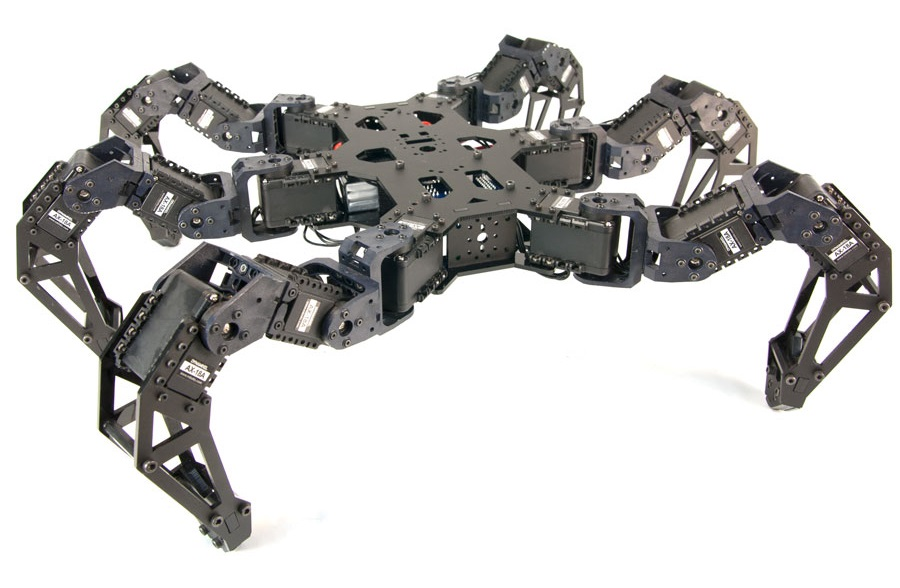
\includegraphics[width=60mm, clip]{figure/chapter2/phantomx_mk2.jpg}
    \caption{PhantomX Mark I\hspace{-1.2pt}I}
    \label{fig:phantomx_mk2} % chktex 24
  \end{center}
\end{figure}

% 脚の座標系
\begin{figure}[h]
  \begin{tabular}{cc}
    \begin{minipage}{0.5\textwidth}
      \centering
      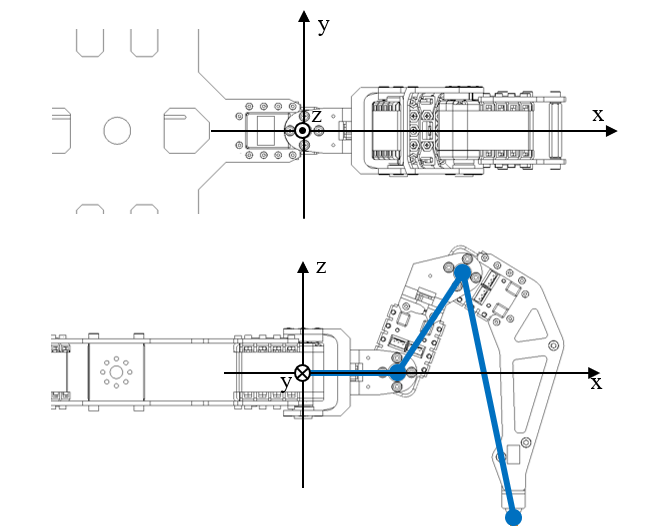
\includegraphics[width=1.0\linewidth]{figure/chapter2/coordinate_axis.png}
      \caption{Leg Coordinate Axis}
      \label{fig:leg_coordinate_axis} % chktex 24
    \end{minipage}
    \begin{minipage}{0.5\textwidth}
      \centering
      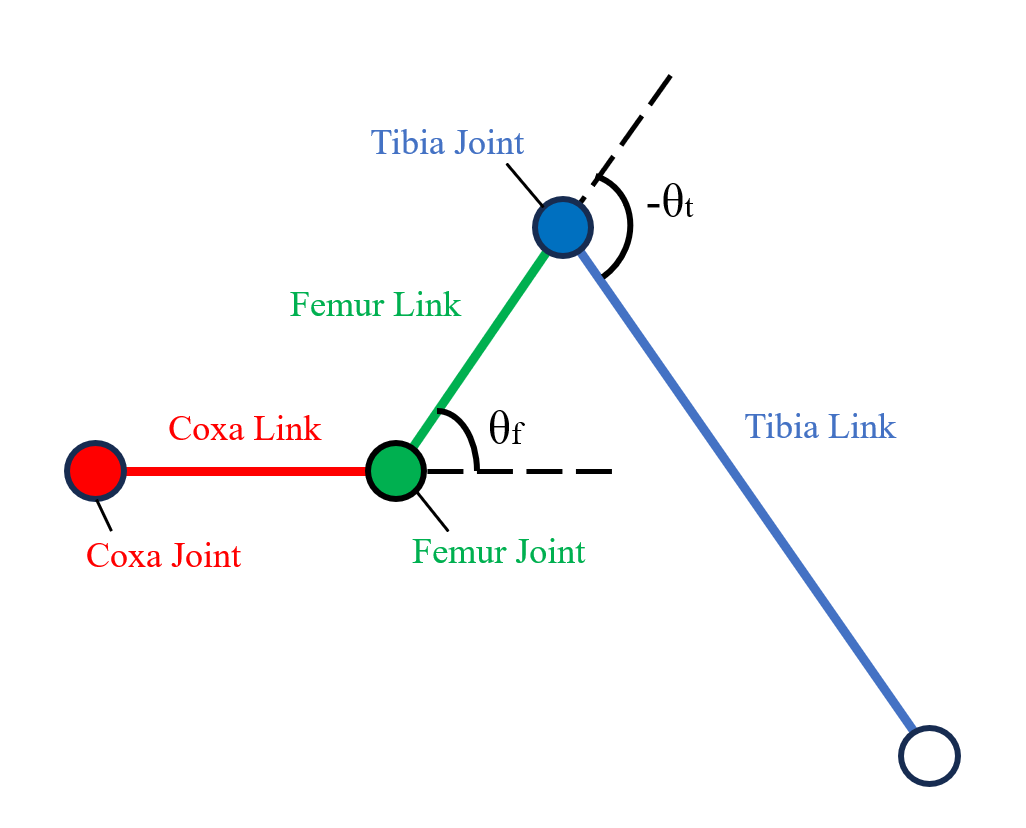
\includegraphics[width=1.0\linewidth]{figure/chapter2/link_joint.png}
      \caption{Joint and Link Name} 
      \label{fig:joint_and_link} % chktex 24
    \end{minipage}
  \end{tabular}
\end{figure}

% 脚長の表
\begin{table}[h]
	\caption{Link Length of PhantomX}
	\label{tab:link_len_phantom_x}  % chktex 24
	\begin{center}
   	\begin{tabular}{|c||c|} \hline  % chktex 44
      Link Name & $[mm]$ \\ \hline  % chktex 44
      Coxa Link & 52  \\ \hline  % chktex 44
      Femur Link & 66  \\ \hline  % chktex 44
      Tibia Link & 130  \\ \hline  % chktex 44
    \end{tabular}
  \end{center}
\end{table}

\newpage

以上の式を用いて,PhantomXの脚の可動範囲を求めたものが\figref{fig:simu_leg_range}である.
\figref{fig:simu_leg_range}では,$\theta_c = 0$とした時の,x-z平面における脚の可動範囲を示している.
横軸をx軸,縦軸をz軸とし,単位は$[mm]$である.
黒色の実線で示される領域が実際の脚の可動範囲であり,緑色の実線で示される領域が近似された脚の可動範囲である.
赤色の点線で示される直線は遊脚の高さを表しており,この直線よりも高く上げることはない.
青色の線と頂点で示される図形は脚の概形である.

\figref{fig:simu_leg_range}より,$100 < x < 150$,$-50 < z < -20$の範囲は,
実際の脚の可動範囲と近似された脚の可動範囲が異なる領域になっているとわかる.
この領域内の点を脚の接地点として選択してしまうと,脚の可動範囲外に脚先が出てしまうため,
脚軌道を生成できず,脚が接地できないことによって転倒してしまう.
また,この領域の点を脚の接地点として選択していなくとも,
脚軌道がこの領域を通過する場合,脚の可動範囲外に脚先が出てしまうため,
矩形軌道の生成に失敗し,この領域を避けるような不完全な脚軌道が生成される.
プログラムは矩形軌道を描くことを前提にしているため,
このような不完全な脚軌道を生成すると,障害物に脚が引っかかってしまい歩行を継続できなくなる.
以上から,この領域が脚軌道生成の失敗の原因であると予想できる.

\figref{fig:simu_leg_range}は遊脚高さを$20 [mm]$,最小半径を$120 [mm]$とした時のものであるが,
遊脚高さを$25 [mm]$,最小半径を$130 [mm]$とした時の脚の可動範囲を\figref{fig:act_leg_range}に示す.
\figref{fig:simu_leg_range}の条件は波東らの研究\cite{Hato_Graph_search}のシミュレーション実験時の条件であり,
\figref{fig:act_leg_range}の条件は実機試験時の条件である.
\figref{fig:act_leg_range}では,$100 < x < 150$,$-50 < z < -20$の範囲の,
実際の脚の可動範囲と近似された脚の可動範囲が異なる領域の大きさが小さくなっていることがわかる.
実機試験時にあたり,条件を変更する必要があったことからも,
近似値と実際の値の差が脚軌道生成失敗に影響していると予想できるだろう.

\newpage

\begin{figure}[h]
  \begin{tabular}{cc}
      \begin{minipage}{0.5\textwidth}
          \centering
          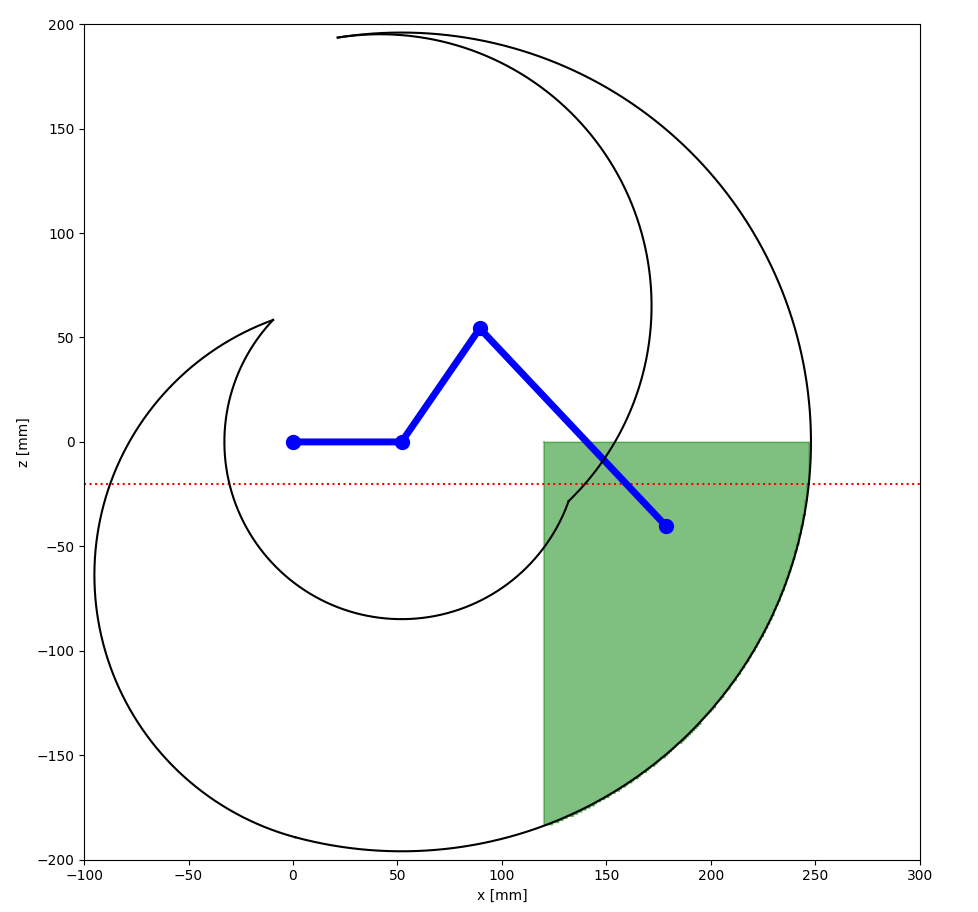
\includegraphics[width=1.0\linewidth]{figure/chapter2/leg_range_120_20.png}
          \caption{Approximated Range of Motion in Simulation \newline}
          \label{fig:simu_leg_range} % chktex 24
      \end{minipage}
      \begin{minipage}{0.5\textwidth}
          \centering
          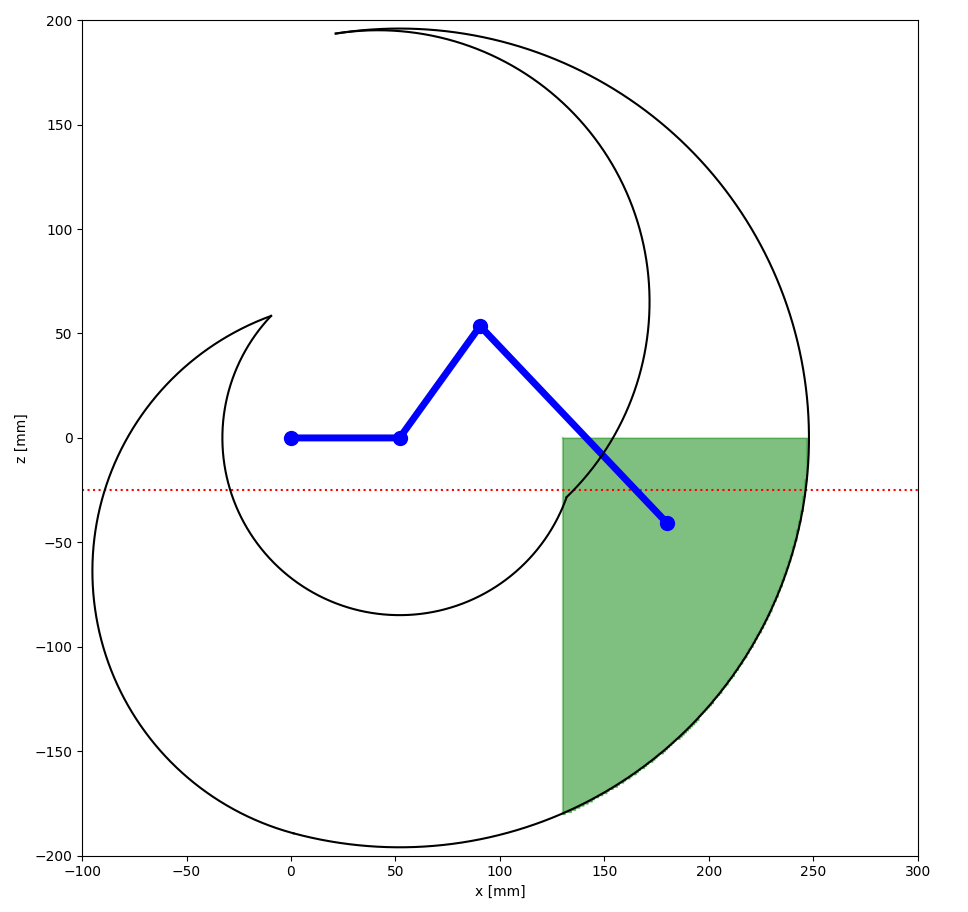
\includegraphics[width=1.0\linewidth]{figure/chapter2/leg_range_130_25.png}
          \caption{Approximated Range of Motion in Experimental Equipment}
          \label{fig:act_leg_range} % chktex 24
      \end{minipage}
  \end{tabular}
\end{figure}

% 予備実験の章
\section{歩行シミュレーションによる脚軌道生成失敗時の脚先位置の特定}

\subsection{シミュレーション実験の目的}
先行研究では脚軌道生成の失敗による動作の停止が報告された上,
その原因は脚先が脚の可動範囲の外を通ることによるものであると考察されてきた.
しかし,具体的にどのような理由で脚軌道生成が失敗するのかは明らかにされていなかった.
そのため予備実験として,波東らの研究\cite{Hato_Graph_search}の実機試験と同じ条件で歩行シミュレーション実験を行う.
実験の目的は脚軌道生成の失敗の回数,接地時の脚位置,そして脚軌道を確認することで,脚軌道生成失敗の原因を特定することとする.

波東らは段差のある地形と斜面のある地形でシミュレーション,および実機による直進歩行動作の実験を行った.
また,実機試験時にはシミュレーション実験と歩行時の条件を変更していた.
本シミュレーションでは,波東らの研究のシミュレーションと実機試験それぞれの条件で歩行シミュレーションを行う.

\subsection{シミュレーションの条件}
本研究室ではロボットの動作のシミュレーションを行うためのシミュレーターソフトウェアを自作し,
シミュレーション実験を行ってきた.
本論文でも同様に,シミュレーション実験に自作のシミュレーターソフトウェアを用いた.

シミュレーターはC++で記述されており,WindowsAPIを用いてGUIを実装し,ロボットを表示している.
また,GUIの表示のプログラムをより簡単に記述するため,
ゲームプログラミングに用いられるライブラリのDxLib\cite{Dxlib_Web}を用いている.
シミュレーターは物理演算を行っておらず,トルク不足や摩擦,脚先の滑りによるずれを考慮していない.
そのため,ロボットのアクチュエータは無限のトルクを持ち,脚先は滑りなく接地するものと仮定している.
本来これらのパラメータを考慮すべきではあるが,
本研究においては歩容パターン生成によって得られた脚接地点に脚先を届かせることが可能であるか確認することが目的であるため,
これらのパラメータは考慮しないこととしている.

\subsubsection{シミュレーションの計算環境}
シミュレーションの計算環境は\tableref{tab:simulation_env}に示した.

\subsubsection{モデルとするロボット}
モデルとするロボットは\figref{fig:phantomx_mk2}のPhantomX Mark I\hspace{-1.2pt}Iとする.

\subsubsection{歩行する地形}
歩行する地形を\figref{fig:terrain}に示す.
地形は5種類あり,それぞれ平地,上り段差,下り段差,上り斜面,下り斜面である.
実機試験の条件に合わせ,段差は上り,下りともに高さが$100 [mm]$とし,
斜面は上り,下りともに角度が$15 [\deg]$とした.

\subsubsection{歩行する時の条件}
シミュレーション時の歩行条件は以下の通りである.
\begin{itemize}
  \item 胴体姿勢は常に水平である.
  \item 最小半径を$120 [mm]$とする.
  \item 重心から見た遊脚高さを$-20 [mm]$とする.
  \item 胴体を地形から最小$30 [mm]$離す.
  \item 常に静的安定余裕は$10 [mm]$以上を保つ.
\end{itemize}

実機実験時の歩行条件は以下の通りである.
\begin{itemize}
  \item 胴体姿勢は常に水平である.
  \item 最小半径を$130 [mm]$とする.
  \item 重心から見た遊脚高さを$-25 [mm]$とする.
  \item 胴体を地形から最小$50 [mm]$離す.
  \item 常に静的安定余裕は$15 [mm]$以上を保つ.
\end{itemize}

以上の2つの条件で歩行シミュレーションを行う.

\subsubsection{シミュレーションの手順}
これらの地形で水平方向に$1200 [mm]$直進させ,
\figref{fig:terrain}のロボットの初期位置をランダムに変化させて計5回ずつ歩行させる.

このシミュレーションでは脚軌道生成に失敗した場合も,
仮に脚軌道生成に成功した場合と同様に歩行を継続させ,
脚軌道生成に失敗した場合の脚先の位置と回数を記録する.
これを各地形,各条件で行う.

% 計算環境の表
\begin{table}[htbp]
	\caption{Simulation Environment}
	\label{tab:simulation_env}  % chktex 24
	\begin{center}
   	\begin{tabular}{|c||c|} \hline  % chktex 44
      CPU & 11thGen Intel Core (TM) i5--11400  \\ \hline  % chktex 44
      RAM & 32.0GB  \\ \hline  % chktex 44
      OS & Windows 11 Home  \\ \hline  % chktex 44
      開発環境 & Visual Studio 2022 Community  \\ \hline  % chktex 44
      使用言語 & C++20  \\ \hline  % chktex 44
    \end{tabular}
  \end{center}
\end{table}

\newpage

% 地形の図
\begin{figure}[htbp]
  \begin{tabular}{cc}
    \begin{minipage}[t]{0.45\hsize}
      \begin{center}
      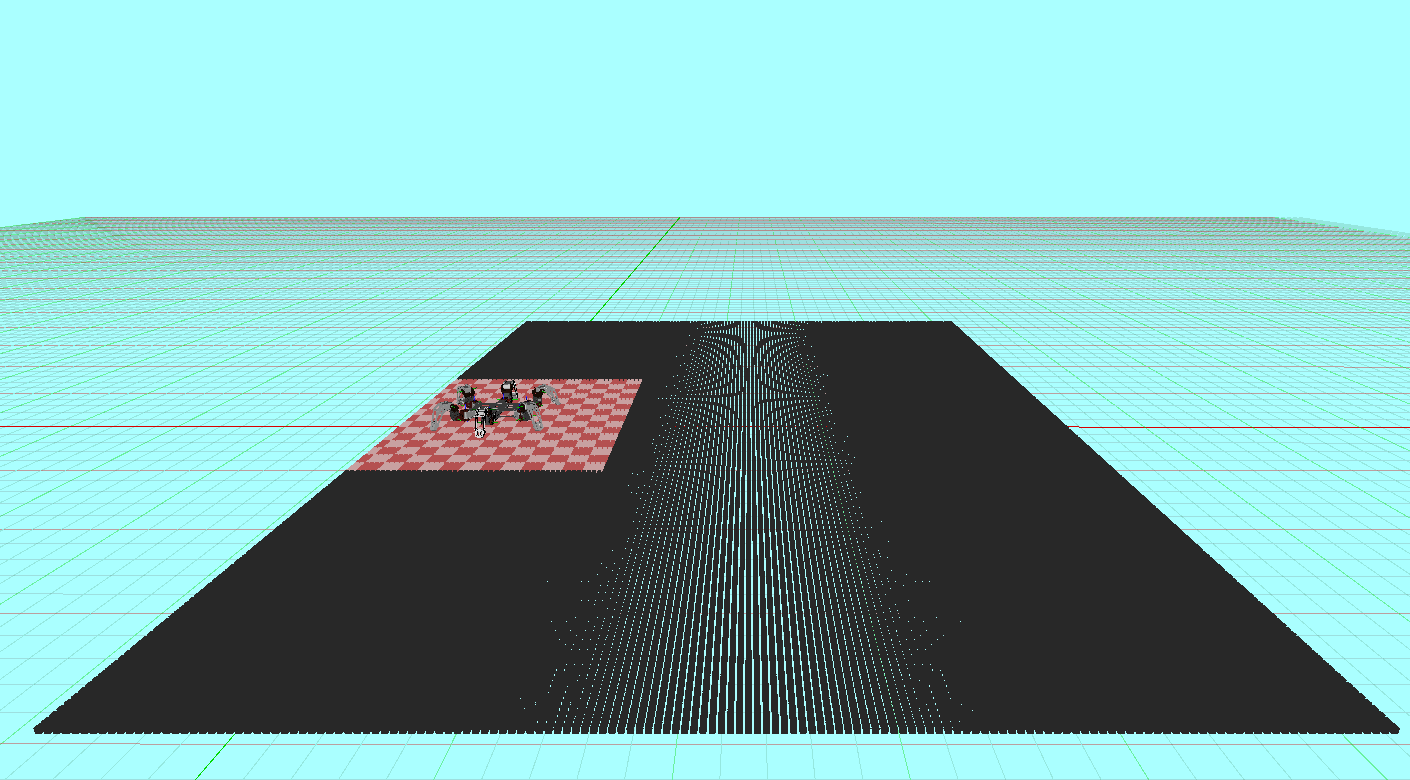
\includegraphics[width=1.0\linewidth]{figure/chapter2/map_flat.png}
      \text{(a) flat}
      \label{fig:flat_terrain} % chktex 24
      \end{center}
    \end{minipage} 
    &
    \begin{minipage}[t]{0.45\hsize}
      \begin{center}
      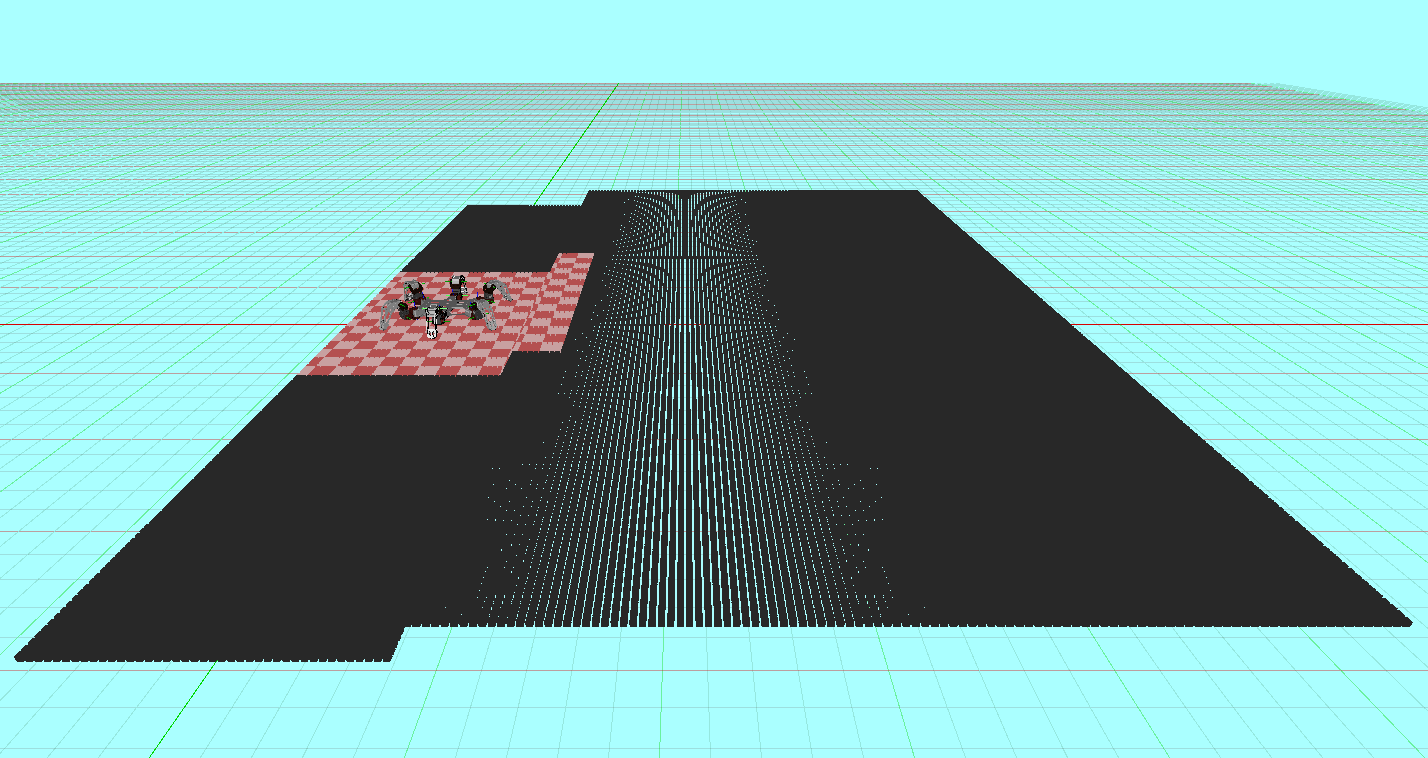
\includegraphics[width=1.0\linewidth]{figure/chapter2/map_100.png}
      \text{(b) up step}
      \label{fig:up_step_terrain} % chktex 24
      \end{center}  
    \end{minipage}
    \\
    &\\  % 空白を入れる
    \begin{minipage}[t]{0.45\hsize}
      \centering
      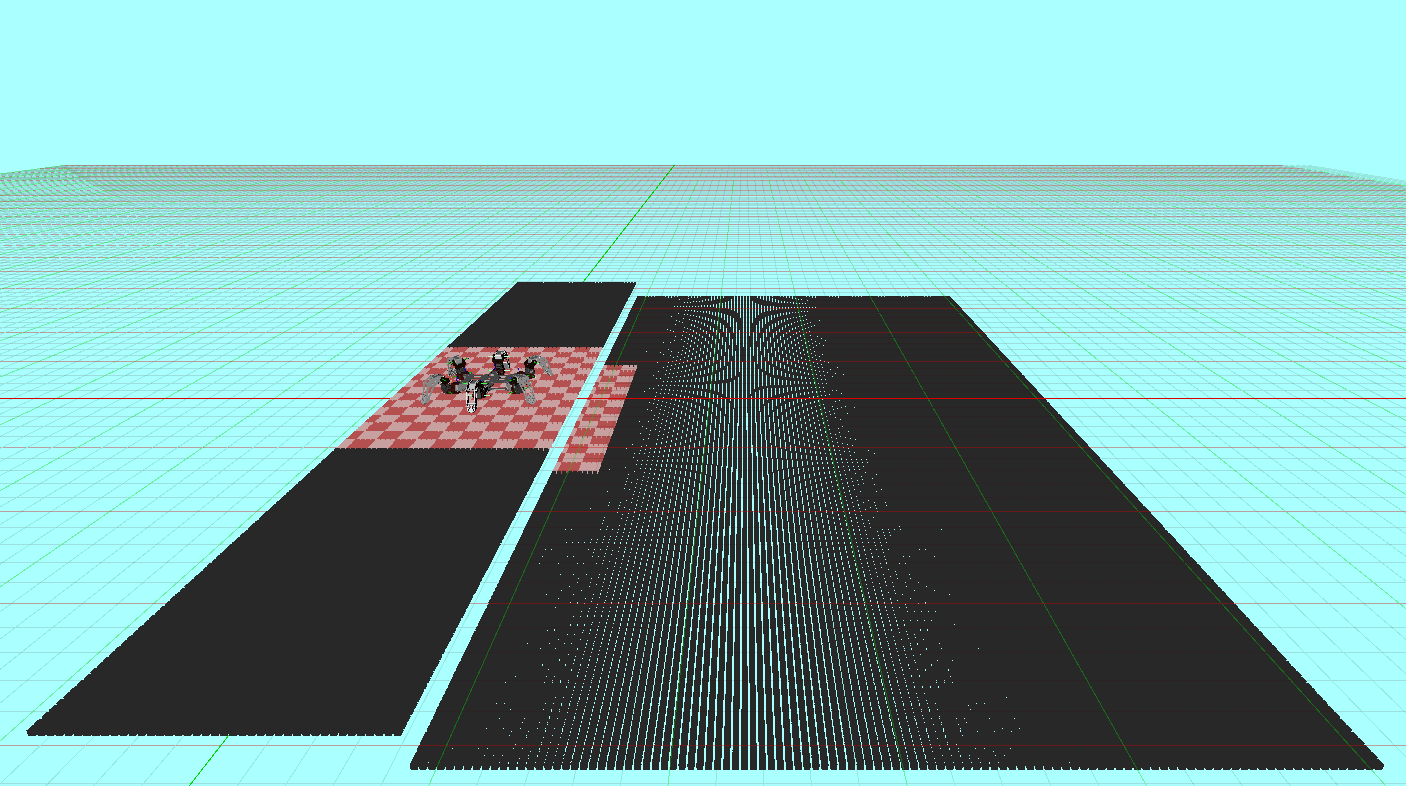
\includegraphics[width=1.0\linewidth]{figure/chapter2/map_-100.png}
      \centering
      \text{(c) down step}
      \label{fig:down_step_terrain} % chktex 24
    \end{minipage} 
    &
    \begin{minipage}[t]{0.45\hsize}
      \centering
      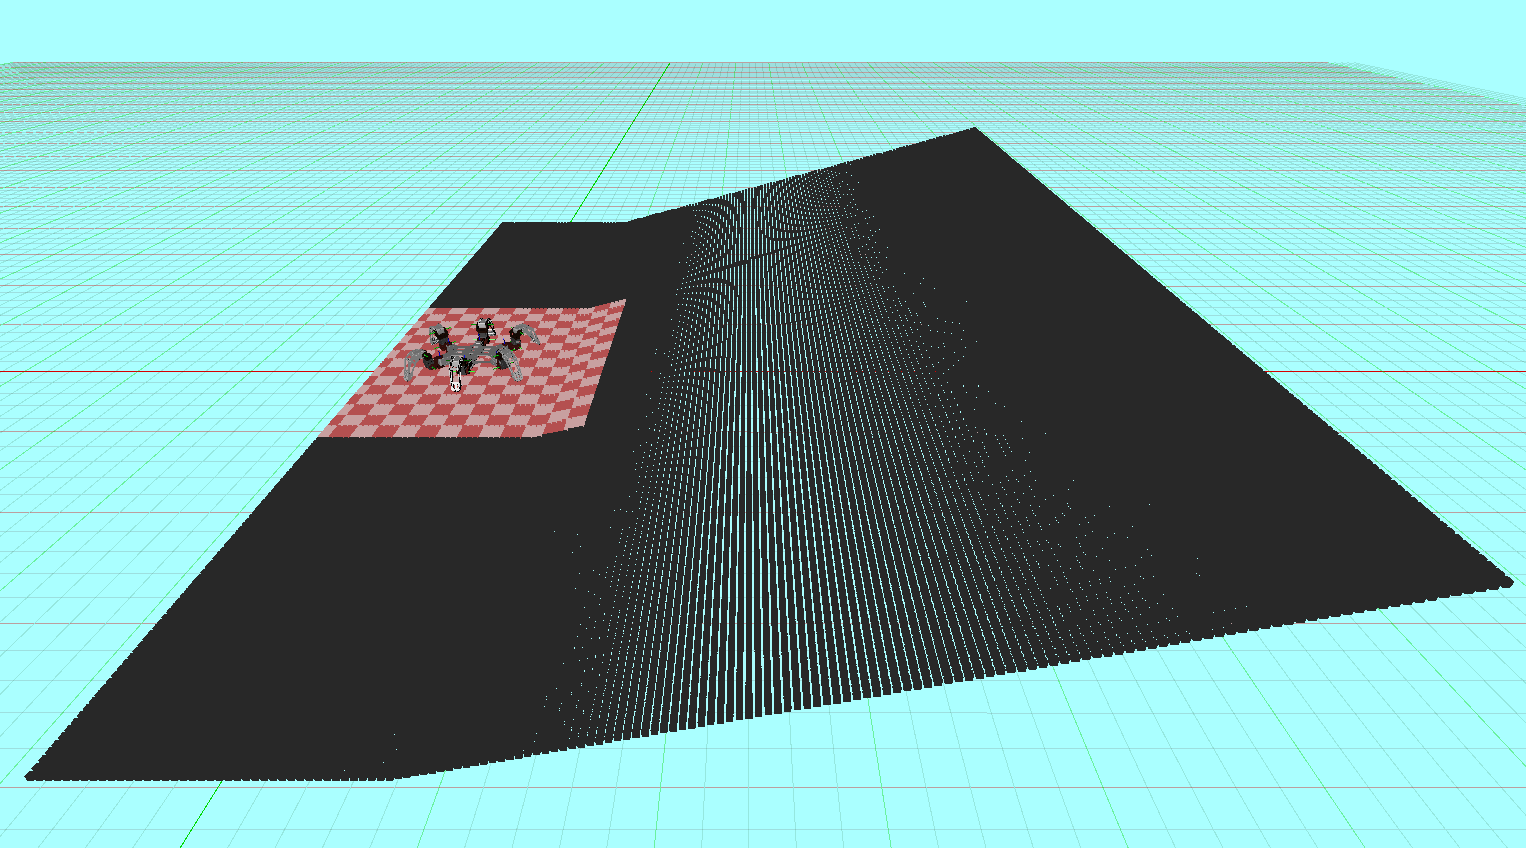
\includegraphics[width=1.0\linewidth]{figure/chapter2/map_15deg.png}
      \centering
      \text{(d) up slope}
      \label{fig:up_slope_terrain} % chktex 24
    \end{minipage}    
    \\
    &\\  % 空白を入れる
    \begin{minipage}[t]{0.45\hsize}
      \centering
      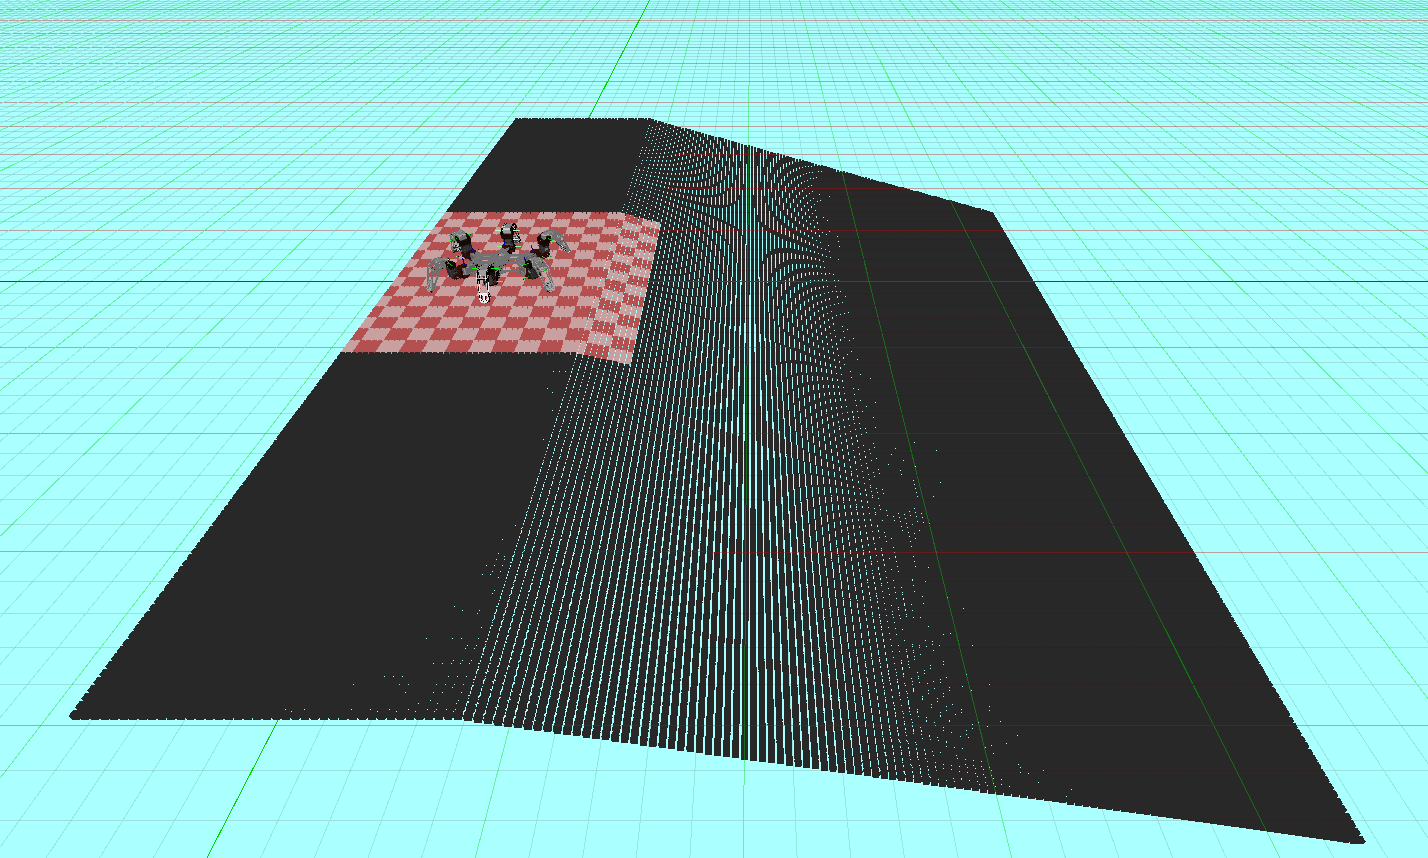
\includegraphics[width=1.0\linewidth]{figure/chapter2/map_-15deg.png}
      \centering
      \text{(e) down slope}
      \label{fig:down_slope_terrain} % chktex 24
    \end{minipage}     
    &
    \\
  \end{tabular}
  \caption{Terrain}
  \label{fig:terrain} % chktex 24
\end{figure}

\newpage

\subsection{シミュレーションの結果}
シミュレーション時の条件で歩行させたときの脚軌道生成失敗の回数を\tableref{tab:failure_count_simulation}に示す.
また,実機実験時の条件で歩行させたときの脚軌道生成失敗の回数を\tableref{tab:failure_count_experimental}に示す.
\tableref{tab:failure_count_simulation}では脚軌道生成の失敗率は多くの地形で$20 [\%]$を超えており,
動作を継続させることが難しいとわかる.
とくに脚の接地点が脚の可動範囲外になってしまうことが多く,
目標の地点まで脚先を届かせることができないため,転倒してしまう可能性が高い.
\tableref{tab:failure_count_experimental}は脚軌道生成の失敗率は多くの地形で$3 [\%]$程度であり,
\tableref{tab:failure_count_simulation}よりも著しく低いことがわかる.
また,脚の接地点が脚の可動範囲外になってしまうことはなく,
目標の地点まで脚先を届かせることができるため,転倒する可能性は低い.
そのため,脚が地形に引っかかってしまわない限り,動作を継続させることが可能であるといえる.


% 書き方 https://uec.medit.link/latex/table.html

\begin{table}[htbp]
  \caption{Failure Count of Simulation}
  \label{tab:failure_count_simulation}  % chktex 24
  \centering
  \begin{tabular}{|c|c|c|c|c|c|c|c|} \hline  % chktex 44
    \multirow{3}{*}{地形} & \multirow{3}{*}{グラフ探索} & \multicolumn{5}{c|}{失敗の回数} & \multirow{3}{*}{失敗率 $[\%]$} \\ \cline{3-7}  % chktex 44
     & & \multirow{2}{*}{脚接地点が} & \multicolumn{3}{c|}{脚軌道が可動範囲外を通る} & \multirow{2}{*}{総失敗} & \\ \cline{4-6}  % chktex 44
     & の回数 & 可動範囲外 & 遊脚時 & 接地時 & \begin{tabular}{c}胴体平行\\移動時\end{tabular} & 回数 & \\ \hline  % chktex 44
    平面     & 315 & 47 & 16 & 4 & 0 & 67 & 21.3 \\ \hline  % chktex 44
    上り斜面 & 460 & 63 & 11 & 22 & 1 & 97 & 21.1 \\ \hline  % chktex 44
    下り斜面 & 611 & 29 & 53 & 28 & 0 & 110 & 18.0 \\ \hline  % chktex 44
    上り段差 & 368 & 50 & 16 & 10 & 0 & 76 & 20.7 \\ \hline  % chktex 44
    下り段差 & 331 & 33 & 39 & 6 & 0 & 78 & 23.6 \\ \hline  % chktex 44
  \end{tabular}
\end{table}

\begin{table}[htbp]
  \caption{Failure Count of Experimental Equipment}
  \label{tab:failure_count_experimental}  % chktex 24
  \centering
  \begin{tabular}{|c|c|c|c|c|c|c|c|} \hline  % chktex 44
    \multirow{3}{*}{地形} & \multirow{3}{*}{グラフ探索} & \multicolumn{5}{c|}{失敗の回数}  & \multirow{3}{*}{失敗率 $[\%]$} \\ \cline{3-7}  % chktex 44
     & & \multirow{2}{*}{脚接地点が} & \multicolumn{3}{c|}{脚軌道が可動範囲外を通る} & \multirow{2}{*}{総失敗} & \\ \cline{4-6}  % chktex 44
     & の回数 & 可動範囲外 & 遊脚時 & 接地時 & \begin{tabular}{c}胴体平行\\移動時\end{tabular} & 回数 & \\ \hline  % chktex 44
    平面     & 351 & 0 & 9 & 2 & 0 & 11 & 3.13 \\ \hline  % chktex 44
    上り斜面 & 645 & 0 & 10 & 1 & 0 & 11 & 1.71 \\ \hline  % chktex 44
    下り斜面 & 867 & 0 & 20 & 9 & 0 & 29 & 3.34 \\ \hline  % chktex 44
    上り段差 & 461 & 0 & 6 & 10 & 0 & 16 & 3.47 \\ \hline  % chktex 44
    下り段差 & 383 & 0 & 9 & 0 & 0 & 9 & 2.35 \\ \hline  % chktex 44
  \end{tabular}
\end{table}

\newpage

シミュレーション時の条件で歩行させたとき,
脚軌道生成に失敗した脚先の位置を\figref{fig:result_of_simulation}に示す.
また,実機実験時の条件で歩行させたとき,
脚軌道生成に失敗した脚先の位置を\figref{fig:result_of_experimental}に示す.
どちらの図も\figref{fig:simu_leg_range}と\figref{fig:act_leg_range}の
$50 < x < 250$,$-200 < z < 0$の範囲を拡大したものである.
橙色の点は脚先が脚の可動範囲外になってしまった時の脚先の位置であり,
青色の点は脚軌道が脚の可動範囲外を通ってしまった時の脚先の位置である.
青色は始点,藍色は終点を表しており,明るい水色は中継点を表している.
それぞれ,すべての地形での結果をまとめて図示している.
この結果から,脚軌道生成に失敗した時の脚先の位置は,
実際の脚の可動範囲と近似された脚の可動範囲が異なる領域を通っていることがわかる.

\begin{figure}[h]
  \begin{tabular}{cc}
      \begin{minipage}{0.5\textwidth}
          \centering
          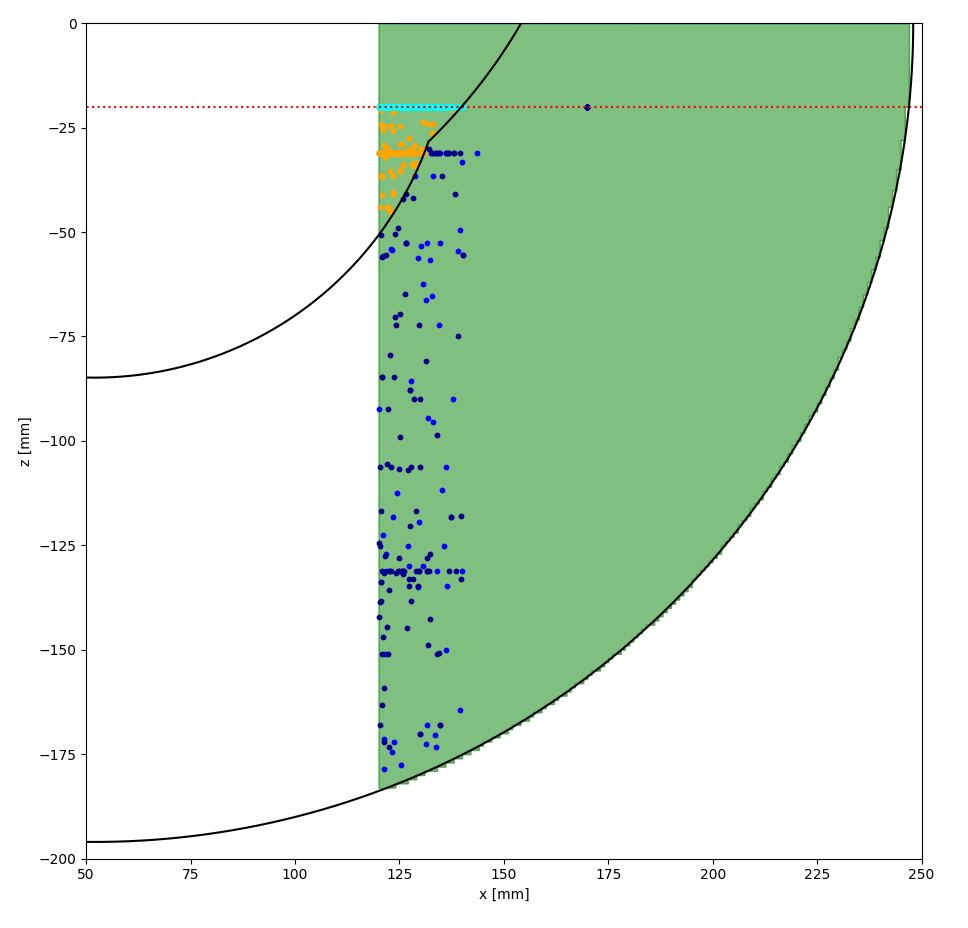
\includegraphics[width=1.0\linewidth]{figure/chapter2/result_simu.png}
          \caption{Result of Simulation}
          \label{fig:result_of_simulation} % chktex 24
      \end{minipage}
      \begin{minipage}{0.5\textwidth}
          \centering
          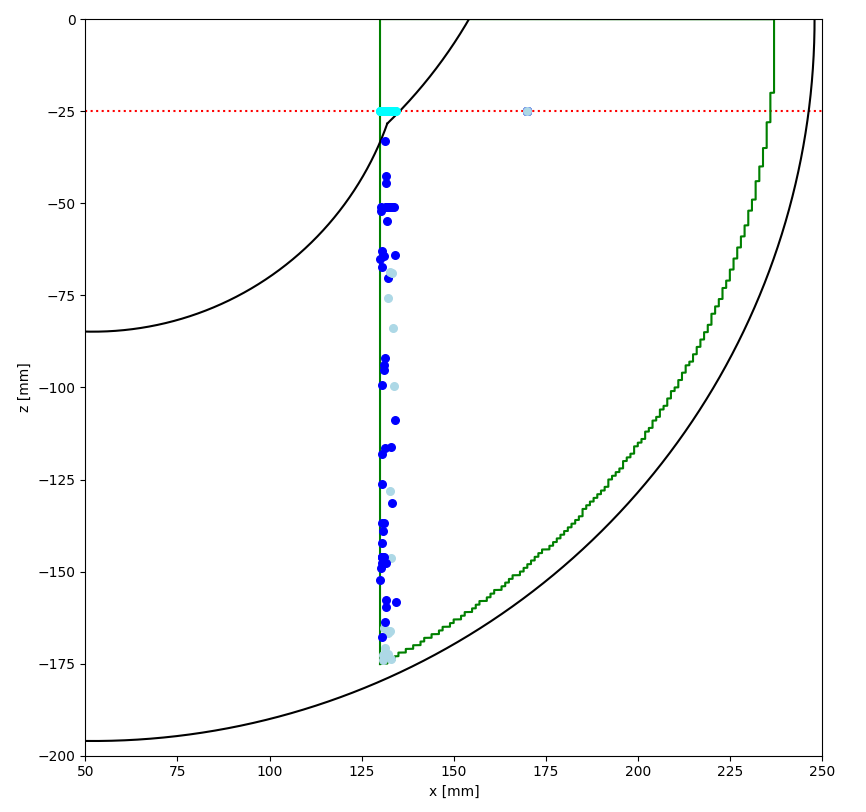
\includegraphics[width=1.0\linewidth]{figure/chapter2/result_exp.png}
          \caption{Result of Experimental Equipment}
          \label{fig:result_of_experimental} % chktex 24
      \end{minipage}
  \end{tabular}
\end{figure}

\subsection{脚軌道生成に失敗する原因の考察}
脚軌道生成に失敗した時の脚先の位置が,
実際の脚の可動範囲と近似された脚の可動範囲が異なる領域を通っていることから,
2.1.3章で予想した通り,実際の脚の可動範囲と近似された脚の可動範囲が異なる領域によって,
脚軌道生成に失敗することがわかった.

% 再評価手法の提案の章
\section{歩容パターンの再評価手法}
脚軌道生成の失敗を防ぐためには近似された脚の可動範囲を小さくするか,
より正確に近似することで誤差をなくせばよい.
しかし,前者は脚の接地点として選択される領域を縮めてしまうことになるため,
グラフ探索による手法の利点である効率的な動作ができなくなってしまうことや,
本来歩行可能であった地形を歩くことができなくなってしまうことなどの問題点がある.
また,後者は細かく正確に近似するとキャッシュしておく値が増えるため,
あらかじめ計算しておいた値にアクセスする際の呼び出しにかかる時間が長くなってしまう.
これにより,計算時間が長くなってしまう問題点がある.

先行研究では,シミュレーション時と実機試験時の条件を変更していたとおり,
前者の方法でこの問題に対応をしていた.
しかし\tableref{tab:walkable_terrain}の歩行条件と,
それを適用したときの歩行可能な地形を示した表からもわかるように,
上り段差と下り段差では歩行可能な地形が変わってしまい,
シミュレーションで歩くことができた地形を歩くことができなくなってしまった.
加えて,この上でも脚軌道生成に失敗してしまうことがあったため,
根本的にこの問題を解決するための方法を考える必要がある.

そこで,歩容パターングラフ探索の再評価を行うことで,脚軌道生成の失敗を防ぐ手法を提案する.
歩容パターングラフ探索の再評価とは,脚軌道生成に失敗した場合,
グラフ探索の処理をやり直して,脚軌道生成に失敗しないような歩容パターンを生成することと定義する.
グラフ探索の再評価の手順を\figref{fig:revaluation_methodolgy}に示す.
再評価手法では基本的には従来手法通りにグラフ探索による歩容パターン生成を行い,
脚軌道生成を行ってロボットを動作させる.
脚軌道生成に失敗した場合のみ,グラフ探索による歩容パターン生成をやり直して,
脚軌道生成に失敗しない新しい歩容パターンを生成する.
歩容パターン生成をやり直す際,脚軌道生成に失敗しないよう,脚の近似された可動範囲を狭め,
可動範囲外に接地することがないようにする.
こうして歩容パターングラフを再生成し,グラフ探索を再度行うことで,
脚軌道生成に失敗しないノードを取得することが可能となる.

再評価手法は前述した2つの解決法と比べ,それらのもつ問題点を克服している.
以下にそれぞれの解決策と比較した再評価手法の利点を示す.

\begin{description}
  \item[本来接地可能だった地点を選択できなくなってしまう問題]\mbox{}\\
    脚の可動域をある程度広く確保することが可能になり,
    可動範囲の境界に近い点を接地点として選択できるようになる.
    加えて,脚軌道生成に失敗する場合,狭められた可動域に切り替えて失敗を防ぐことができる.
    \\
  \item[値を呼び出す際にかかる時間が増えてしまう問題]\mbox{}\\
    再評価手法では歩容パターン生成をやり直す都合上,
    単純計算で探索にかかる時間が倍になってしまう.
    よってより正確に近似する方が実行時間的に優れると思える.
    しかし,歩容パターングラフの生成時には $10^5 \sim 10^6$ 程度の数のノードを生成するため,
    グラフ探索内の処理の時間の増加は,最終的な計算時間を大幅に増加させてしまう可能性がある.
    つまり再評価手法では計算時間の増加を約 2 倍程度で済ませることができるといえる.
\end{description}

\begin{table}[h]
	\caption{Walkable Terrain}
	\label{tab:walkable_terrain}  % chktex 24
	\begin{center}
   	\begin{tabular}{|c|c|c|} \hline  % chktex 44
      地形 & シミュレーション時 & 実機実験時 \\ \hline  % chktex 44
      上り段差 & $130 [mm]$ & $100 [mm]$ \\ \hline  % chktex 44
      下り段差 & $-130 [mm]$ & $-100 [mm]$\\ \hline  % chktex 44
      上り斜面 & $15 [\deg]$ & $15 [\deg]$ \\ \hline  % chktex 44
      下り斜面 & $-15 [\deg]$ & $-15 [\deg]$ \\ \hline  % chktex 44
    \end{tabular}
  \end{center}
\end{table}

% phantomx mk - 2 の図
\begin{figure}[h]
  \begin{center}
    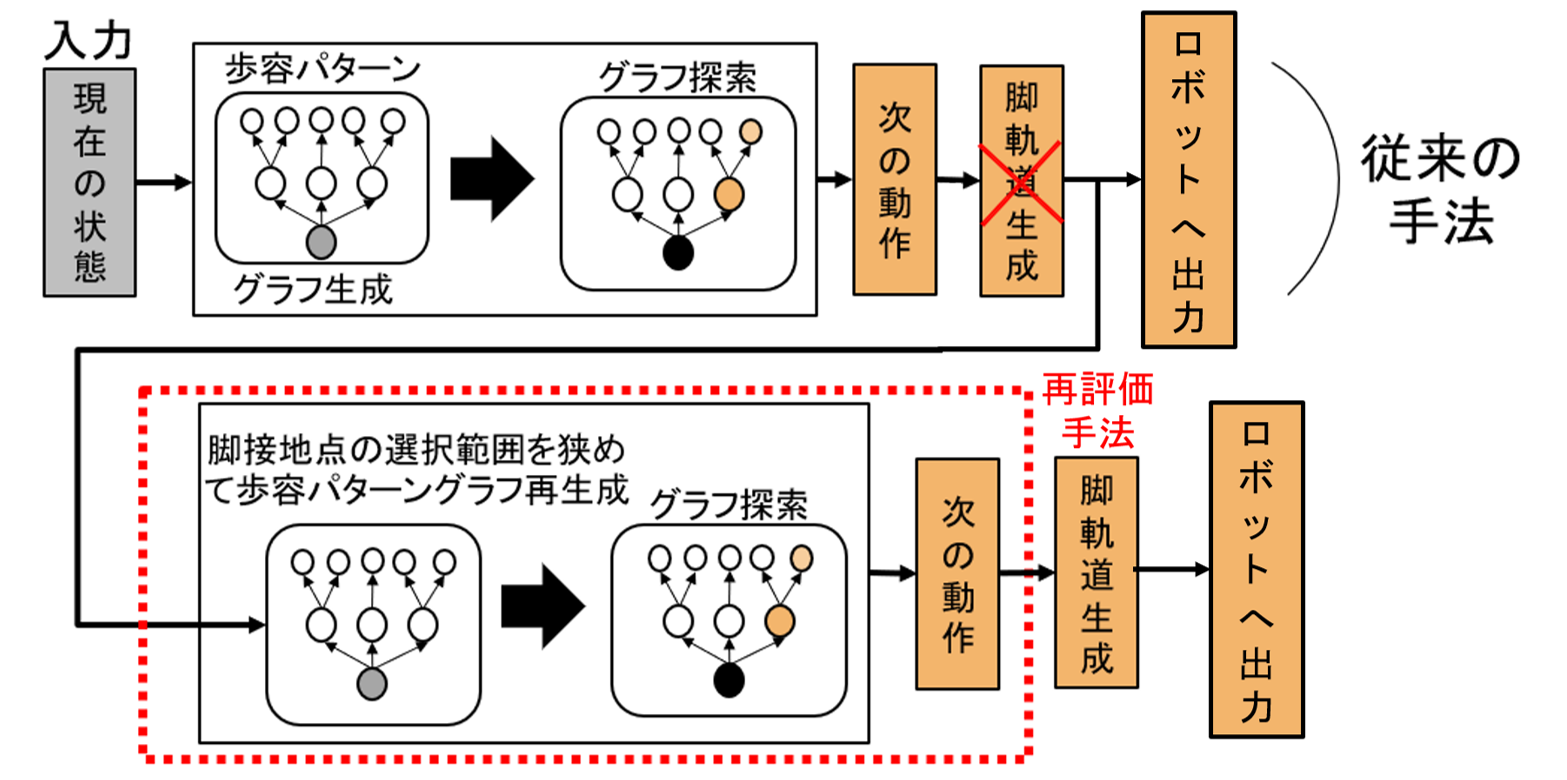
\includegraphics[width=140mm, clip]{figure/chapter2/revaluation_method.png}
    \caption{Revaluation Methodology Procedures}
    \label{fig:revaluation_methodolgy} % chktex 24
  \end{center}
\end{figure}
